%%%%%%%%%%%%%%%%%%%%%%%%%%%%%%%%

% Meta-alignment of Biological Sequences

%%%%%%%%%%%%%%%%%%%%%%%%%%%%%%%%

\chapter[Meta-alignment of Biological Sequences]{\textbf{M}eta-alignment of\\ Biological Sequences}\label{sec:meta}
\sectiongreen*{Summary}
\begin{center}
\begin{tabular}{c}
\fcolorbox{blue}{verylightgrey}{
\begin{minipage}[][4cm][c]{0.8\linewidth}
\sffamily
%abstract 
This chapter contains the description of an efficient algorithm to align higher
order elements mapped over biological sequences. The relationship between
sequence alignments and meta-alignment is also reviewed. Such an approach 
is trained on a set of well annotated promoters. The ability of the meta-alignment 
to identify functional elements conserved at high level, such as regulatory elements
in co-regulated genes, in absence of sequence conservation is shown in several situations. 
In addition, the meta-alignment is used to evaluate the specificity of the weight matrices 
in a genome wide approach.
\end{minipage}}\\
\\[2ex]
\begin{minipage}[][4cm][c]{1.1\linewidth}
\minitoc
\end{minipage}
\end{tabular}
\end{center}
\newpage

\sectiongreen{Biological maps: promoters}\label{sec:}

\lettrine[lines=4,loversize=-0.1,lraise=0.1,lhang=.2]{S}{equence comparisons 
\index{sequence!seqcmp@sequence comparison} are among 
the most useful computational techniques} in molecular biology. Sequences of characters 
in the four-letter nucleotide alphabet and in the twenty-letter amino acid alphabet are 
extremely good symbolic representations of the underlying DNA and protein
molecules, and encode substantial information on their structure, function 
and history. 

Primary sequence comparisons, however, have limitations. Although 
similar sequences do tend to play similar functions, the opposite 
is not necessarily true. Often similar functions are encoded in
higher order sequence elements --such, for instance, structural motifs 
in amino acid sequences-- and the relation between these and the 
underlying primary sequence may not be univocal. As a result, similar 
functions are frequently encoded by diverse sequences.

As reviewed in Chapter \ref{sec:algorithms}, a biological map \index{maps}
is a description of functional objects (e.g. genes or regulatory sites) that are identified in a 
sequence at a given position. The annotation of the human genome in Figure \ref{fig:hgenome}
\index{genome!humgen@human genome} is a clear example of genomic mapping \index{genomic mapping} 
\citep{venter:2001a}. Comparison operations between maps are 
then necessary to elucidate functional relationships that are undetectable at the sequence level.

Promoter regions controlling eukaryotic gene expression are a case in
point. As reviewed in Chapter \ref{sec:genefinding}, the information for the control of the 
initiation of the gene transcription is mostly contained in the gene promoter, a region 
upstream of the gene transcription start site (TSS). Transcription factors
(TFs) interact in these regions with sequence specific elements or motifs 
(the TF binding sites, TFBSs). TFBSs are typically 5-15 nucleotides long and 
one promoter region usually contains many of them to harbor different TFs 
\citep{wray:2003a}. The interplay between these factors is not well understood, but the motifs 
appear to be arranged in specific configurations that confer on each gene an individualized
spatial and temporal transcription program \citep{wray:2003a}. It is
assumed, in consequence, that genes exhibiting similar expression
patterns would also share similar configurations of TFs in their
promoter.

However, TFBSs associated to the same TF are known to tolerate
sequence substitutions without losing functionality, and are often not
conserved.  Consequently, promoter regions of genes with similar
expression patterns may not show sequence similarity, even though they
may be regulated by similar configurations of TFs. For instance, only
about 30 to 40\% of the promoter regions are conserved between human
and chicken orthologous genes \citep{hillier:2004a}, and the
conservation of human-mouse orthologous promoter regions is only
slightly higher than that observed in intergenic regions
\citep{waterston:2002a}. Indeed, despite the recent progress due to the
development of techniques based in the so-called phylogenetic
footprinting, lack of nucleotide sequence conservation between functionally 
related promoter regions may partially explain the still limited success of 
current available computational methods for promoter characterization 
(see Chapter \ref{sec:genefinding} for a review of these methods).

%%%%
% Figure 1: the human genome is a map
%%%%
\begin{figure}[t!]
\begin{center}
\setlength{\fboxsep}{0pt}
\fbox{\incgraph{width=0.9\linewidth}{ps/hgenome}}
\mycaption{fig:hgenome}% label
          {The human genome map}% lof
          {The human genome map.}% caption header
          {This poster was produced with the program \prog{gff2ps} \citep{abril:2000a}. 
           Adapted from \citet{venter:2001a}.}
\end{center}
\end{figure}

In the approach described in this chapter \citep{blanco:2006b}, 
we attempt to overcome this limitation
by abstracting the nucleotide sequence, and representing a promoter
region by a sequence in a new alphabet in which the different symbols
denote different TFs. Using an external mapping function (for instance, 
a look-up table or a collection of position weight matrices, PWMs) that 
associates each TF to the nucleotide sequence motifs the factor is
known to bind, we can translate the nucleotide sequence of the
promoter into a sequence in this new alphabet. These sequences 
can be aligned. If the scoring of the
alignment takes into account not only the presence/absence of a given
symbol, but its relative position on the primary nucleotide sequence,
the optimal alignment between the promoter regions of two 
genes with similar expression patterns 
may reflect the underlying common configuration of
TFBSs.  We refer to these alignments either as meta-alignments, \index{meta-alignments}
as they are performed between sequences in a meta-alphabet, or map
alignments, since they are obtained after mapping the nucleotide
sequence in a higher order alphabet.

\sectiongreen{Transcription Factor maps}\label{sec:tfmaps}

Analogously to the restriction enzyme maps initially formalized by 
\citet{waterman:1984c} that are described in Chapter \ref{sec:algorithms},
we translate in our approach \citep{blanco:2006b} the nucleotide sequence 
of a promoter region $S = s_1 s_2 \ldots s_k$  into a sequence of 4-tuples
$A = a_1 \ldots a_n$ where each $a_i = <a_i^f,a_i^{p_1},a_i^{p_2},a_i^s>$
denotes the match with score $a_i^s$ of a binding site for the TF
$a_i^f$  occurring between the position $a_i^{p_1}$ and the position
$a_i^{p_2}$ over the sequence $S$. 

We obtain the translation from $S$ to $A$ by running on $S$ a collection of 
PWMs representing binding motifs for TFs (such as, for instance, the collection 
in \db{Transfac} \citep{matys:2003a}). For each match over a given threshold, we
register in $A$ the positions ($a_i^{p_1},a_i^{p_2}$), the score
($a_i^s$), and the label ($a_i^f$) of the TF associated to the PWM.
The translation preserves the order of $S$ in $A$, that is if $i < j$
in $A$ then $a_i^{p_1} \leq a_j^{p_1}$ (the $\leq$ is because matches
to different TFs may occur at the same position). We will refer to the
resulting sequence $A$ as a Transcription Factor Map (TF-map) 
\index{maps!tf@TF-maps} \index{TF-maps} or simply a map (see Figure 
\ref{fig:dummy}).  Note that other mapping functions, instead of
collections of PWMs, can also be used to translate $S$ into $A$.

In the implementation here, matches to PWMs are considered strandless,
that is, they are annotated at a given location, irrespective of the
orientation in which they occur. While biological evidence 
suggests that some TFBSs are functional only when present in a given 
strand, in other cases TF activity appears to be independent
of the orientation of the binding site \citep{strachan:1999a}. 
Since in general, we do not have information of
the strand in which a binding site may be functional, we have not
considered strand in our analysis.

\sectiongreen{TF-map pairwise alignment}\label{sec:TF-map alignment}

\index{TF-maps!alntf@alignments} \index{TF-map alignments} 
\index{alignment!tfma@TF-map alignments} \index{alignment!meta@meta-alignments}
The same types of sequence alignments that were reviewed in Chapter \ref{sec:algorithms} 
are also possible with maps: pairwise or multiple, global or local alignments. 
In this chapter, we described the algorithms of global and local pairwise TF-map alignment. 
The approach for multiple map alignment is detailed in the next chapter.

\clearpage
Formally, the pairwise alignment of the TF-maps $A = a_1 \ldots a_m$ and $B = b_1 \ldots b_n$ is a 
correspondence $T$, maybe empty, between $A$ and $B$ such that \citep{blanco:2006b}:
\begin{enumerate}

\item $(a_i,b_j) \in T$ if and only if $a_i^f = b_j^f$ (that is,
two elements are aligned if and only if they correspond to the same
TF). 

\item if $(a_i,b_j) \in T$ then there are no other elements $b_l~(l \neq j)$ in
$B$ such that $(a_i,b_l) \in T$, nor elements $a_k~(k \neq i)$ in $A$  such that
$(a_k,b_j) \in T$ (that is, each element in $A$ is aligned at most
to one element in $B$, and vice versa).

\item if $(a_i,b_j) \in T$ and $(a_k,b_l) \in T$ and $i<k$ then
$j<l$ (that is, the alignment maintains the colinearity between the
sequences $A$ and $B$).

\item if $(a_i,b_j) \in T$ and $(a_k,b_l) \in T$ with $i<k$ and $j<l$ then
$a_i^{p_2} < a_k^{p_1}$ and $b_j^{p_2} < b_l^{p_1}$ (that is, no overlap
in the primary sequences is permitted between the sites corresponding to the aligned elements).
\end{enumerate}

Usually there are many possible alignments between two given $A$ and
$B$ maps (see Figure \ref{fig:dummy} for an example). Given an alignment $T$

\begin{center}
\fcolorbox{white}{verylightgreen}{
\begin{minipage}[][][c]{0.95\linewidth}
\begin{equation}
T = \{ (a_{I_1},b_{J_1}), (a_{I_2},b_{J_2}), \cdots, (a_{I_t},b_{J_t}) \}
\end{equation}
\end{minipage}}
\end{center}

where $T_k = (a_{I_k},b_{J_k})$ is the match between the 4-tuple in position
${I_k}$ from A and the 4-tuple in position ${J_k}$ from B, we compute
the score of the alignment $s(T)$ in the following way:

\begin{center}
\fcolorbox{white}{verylightgreen}{
\begin{minipage}[][][c]{0.95\linewidth}
\begin{equation}
\begin{array}{ll}
s(T) = & \alpha \sum_{k=1}^t a_{I_k}^s + b_{J_k}^s\\
 & - \lambda (m + n -2 t)\\
%\sum_{k=2}^t (I_k - I_{k-1} - 1) + (J_k - J_{k-1} - 1) \\
 & - \mu \sum_{k=2}^t |(a_{I_k}^{p_1} - a_{I_{k-1}}^{p_1}) - (b_{J_k}^{p_1} - b_{J_{k-1}}^{p_1})|
\end{array}
\end{equation}
\end{minipage}}
\end{center}

where $\alpha, \lambda, \mu > 0$.
That is, the score of the alignment increases with the score of the
aligned elements ($\alpha$), and decreases with the number of
unaligned elements ($\lambda$), and with the difference in the distance 
between adjacent aligned elements ($\mu$).

%%%%
% Figure 2: TF-mapping and dummy TF-map alignment
%%%%
\begin{figure}[t!]
\begin{center}
\setlength{\fboxsep}{0pt}
\fbox{\incgraph{width=0.85\linewidth}{ps/dummy}}
\mycaption{fig:dummy}% label
          {TF-maps: construction and alignment}% lof
          {TF-maps: construction and alignment.}% caption header
          {(A) The sequence of a promoter is searched for occurrences of known
binding motifs for transcription factors (TFs). Matches are annotated with
the position of the match in the primary sequence, and the label of
the TF. Because TFs can bind to
motifs showing no sequence conservation, labels of the same
TF at different positions may correspond to
different underlying nucleotide sequences. We refer here to these
sequences of pairs (``label'', ``position''), transcription factor
maps (or TF-maps). TF-maps are actually more complicated. First, we do
not only register the position of each match, but also its
length. Second, while in the example here, sequence motifs
are associated to TFs by means of a (binary) look-up table, in our
work we have instead used collections of position weight
matrices. Matches to transcription factor binding sites (TFBSs) are thus
scored, and this score is also registered.
(B) TF-map of the promoter region of two hypothetically co-regulated genes
$X$ and $Y$.
Each letter corresponds to a different TF. We assume
that 200 nucleotides upstream of the annotated transcription start site 
(TSS) have been considered, with position 1 corresponding to position 
-200 from the TSS.
(C) Global pairwise alignment of the two co-regulated genes $X$ and $Y$. 
Only positions with identical labels can be aligned. Essentially, the 
alignment finds the longest common substring constrained to maximizing the 
sum of the scores (not shown here) of the aligned positions, and minimizing 
the differences in the distances on the primary sequence between 
adjacent aligned positions.}
\end{center}
\end{figure}

\subsectionblue{Finding the optimal alignment}

The optimal alignment between two given maps $A$ and $B$ is the
one scoring the maximum among all possible alignments. To obtain such
an alignment efficiently, we have implemented an algorithm reminiscent
of that proposed by \citet{waterman:1984c} to align and compare
restriction enzyme maps. This algorithm was developed to find the
distance between two homologous restriction maps in terms of minimum
weighted sum of genetic events necessary to convert one restriction
map into another, where the genetic events are the
appearance/disappearance of restriction sites and changes in the
number of bases between restriction sites (see Chapter \ref{sec:algorithms}
for further details).

Here to align TF-maps $A$ and $B$, we adapted the recursion in
\cite{waterman:1984c} to optimize similarity instead \citep{blanco:2006b}. In addition, we
included a term ($\alpha$) into the scoring function to weight the scores of the
TFBSs. We also explicitly prohibited overlap between the sites.

Thus, the maximum similarity $S_{ij}$ between TF-maps  $A = a_1 \ldots a_i$ and 
$B = b_1 \ldots b_j$ where the site $a_i^f$ is equal to the site $b_j^f$, 
can be computed as: 

\begin{center}
\fcolorbox{white}{verylightgreen}{
\begin{minipage}[][][c]{0.95\linewidth}
\begin{equation}
\begin{array}{llll}
S_{ij} \equiv & S(a_i,b_j) = & \alpha (a_i^s + b_j^s) +& \\
              & &  max_{i',j'} & \{S_{i'j'}\\
              & & \scalebox{0.7}{\mbox{$0 < i' < i$}} & - \lambda (i - i' - 1 + j - j'- 1)\\
              & & \scalebox{0.7}{\mbox{$0 < j' < j$}} & - \mu (|(a_i^{p_1} - a_{i'}^{p_1}) - (b_j^{p_1} - b_{j'}^{p_1})|)\}.\\
              & & \scalebox{0.7}{\mbox{$a_{i'}^{p_2} < a_i^{p_1}$}} & \\
              & & \scalebox{0.7}{\mbox{$b_{j'}^{p_2} < b_j^{p_1}$}} &  
\end{array}
\end{equation}
\label{eqnaive}
\end{minipage}}
\end{center}

\subsectionblue{Sequence alignments and meta-alignments}

\index{TF-map alignments!seqaln@sequence alignments} \index{alignment!seqtf@sequences and TF-maps}
There is an intimate relationship between the Equation \ref{eqnaive} and the Needleman
and Wunsch recurrence as revisited by \citet{smith:1981b} in which the conventional pairwise 
sequence alignment is based (see Chapter \ref{sec:algorithms}, Section \ref{nwrevisited}).

In fact, the sequence alignment class of algorithms are a particular case of the
more general class of map alignment algorithms. Let us analyze the form in which
the conventional sequence alignment calculates any value in the similarity matrix $S$, trying
to detect for each element in such a recurrence its counterpart in Equation \ref{eqnaive}:

\begin{menumerate}
\item
The matches and the substitutions between two symbols $x$ and $y$ are assigned the value 
of the corresponding scoring function $s(x,y)$ in a sequence alignment. The matches between
two elements in a meta-alignment are also scored using a similar function (the $\alpha$ 
parameter in Equation \ref{eqnaive}). Let us consider $\alpha=(\alpha_1,\alpha_2 \ldots \alpha_k)$
the family of scoring functions for evaluate any type of identity and substitution between two
symbols $x$ and $y$. If the mapping quality score of each element is omitted, the scoring functions 
$s$ and $\alpha$ are equivalent.
\item
The number of gaps in a sequence alignment is punished by the scoring function $s(x,-)=s(-,x)$. 
There is not an explicit penalty for introducing a single gap into a meta-alignment. However, 
the $\lambda$ parameter punishes the number of elements in two maps that are not included
in the optimal met-alignment. Because such unaligned elements are implicitly aligned to gaps in 
the other map, the $\lambda$ parameter is the equivalent of the scoring function $s(x,-)$.
\item
The $\mu$ parameter must be silenced due to the lack of mapping information in conventional sequences. 
\end{menumerate}

A trivial mapping function to translate a sequence of nucleotides into a map that can be meta-aligned
consists on using the position of the elements in the sequence also as the position in the map. 
The length of every feature is in this case one position. The score of each feature is neglected
as nucleotides do not have this value. With these considerations in mind, the sequence of nucleotides 
$S=ATTACTG$ can be transformed into the map $M$:

\begin{center}
\fcolorbox{white}{verylightgreen}{
\begin{minipage}[][][c]{0.95\linewidth}
$$%\begin{equation}
\begin{array}{lccccccc}
S: & A & T & T & A & C & T & G\\[2ex]
M: & (A,1,1,\cdot) & (T,2,2,\cdot) & (T,3,3,\cdot) & (A,4,4,\cdot) & (C,5,5,\cdot) & (T,6,6,\cdot) & (G,7,7,\cdot).\\
\end{array}
$$%\end{equation}
\end{minipage}}
\end{center}

The meta-alignment class of algorithms can deal, therefore, with any sequence alignment problem.
However, the opposite is not true, as meta-alignments involve management of higher-order level
features that are not supported in the classical sequence comparisons.


\subsectionblue{Naive implementation}
\index{TF-map alignments!naive@naive algorithm} \index{algorithms!tfnaive@TF-map alignment}
A naive implementation of the recursion above (Equation \ref{eqnaive}) involves
the recursive filling of the cells $S_{ij}$ in the matrix $S$ \citep{waterman:1984c}. 
In the pseudocode shown in Figure \ref{fig:naivealg}, the elements of the maps $A$ and $B$ are represented as 
structures $a_i$ and $b_j$, with the functions \emph{factor}, \emph{score}, \emph{pos1} 
and \emph{pos2} returning the values of the corresponding fields. The variable 
\emph{currentSim} stores the optimal score so far computed. The resulting meta-alignment 
can be easily retrieved using a supplementary structure \emph{path(i,j)} which points to 
the previous cell in the optimal path leading to cell $S_{ij}$. In addition, for each 
cell $S_{ij}$, the function \emph{ComputeInitialSimilarity} calculates the initial score of 
a hypothetical alignment that includes only $a_i$ and $b_j$.

Note that to compute the optimal score at $S_{ij}$ with this algorithm, 
all the cells $S_{kl}$ ($k<i$, $l<j$) need to be explored (see Figure \ref{fig:naivealg}). 
Therefore, if the lengths of the TF-maps $A$ and $B$ are $m$ and $n$ respectively, the 
cost of computing $S(A,B)=S(a_m,b_n)$ is $O(mn \cdot mn) = O(m^2n^2)$. 
Under the assumption that $m$ and $n$ are similar lengths, the final cost 
function is $O(n^4)$.


%%%%
% Figure 3: Naive algorithm
%%%%
\begin{figure}[t!]
\begin{center}
\scalebox{1}{
\fcolorbox{white}{verylightgreen}{
\begin{minipage}[][][c]{0.95\linewidth}
\begin{algorithmic}[5]
 \REQUIRE $A,B$: list of $<$factor,pos1,pos2,score$>$
\STATE \COMMENT{Calculating the element $i,j$ in $S$}
\FOR{$i=0$ to $|A|-1$}
\FOR{$j=0$ to $|B|-1$}
\IF{factor$(a_i)$ = factor$(b_j)$}
\STATE $S(i,j) \leftarrow$ ComputeInitialSimilarity();
\STATE $x \leftarrow \alpha$ (score$(a_i)$ + score$(b_j)$);
\STATE \COMMENT{Searching the best previous match in $S$}
\FOR{$i'=0$ to $i-1$}
\FOR{$j'=0$ to $j-1$}
\IF{pos2($a_{i'}$) $<$ pos1($a_i$) and pos2($b_{j'}$) $<$ pos1($b_j$)}
\STATE $y \leftarrow \lambda ((i-i'-1) + (j-j'-1))$;
\STATE $z \leftarrow \mu (|($pos1$(a_i)$ - pos1$(a_{i'})$) - (pos1$(b_j)$ - pos1$(b_{j'}))|)$;
\STATE currentSim $\leftarrow S(i',j') + x - y - z$;
\IF{currentSim $> S(i,j)$}
\STATE $S(i,j) \leftarrow$ currentSim; 
\ENDIF
\ENDIF
\ENDFOR
\ENDFOR
\ENDIF
\ENDFOR
\ENDFOR
\end{algorithmic}
\begin{center}
%\fbox{
\incgraph{width=0.75\linewidth}{ps/prev}%}
\end{center}
\end{minipage}}}
\mycaption{fig:naivealg}% label
          {The Naive TF-map alignment algorithm}% lof
          {The Naive TF-map alignment algorithm.}% caption header
          {The whole matrix must be visited for each new match $S_{ij}$}
\end{center}
\end{figure}

\subsectionblue{Enhanced implementation}

\index{TF-map alignments!enh@enhanced algorithm} \index{algorithms!tfnaive@TF-map alignment}
\citet{myers:1992a} described an improved algorithm for computing in
$O(mn(\log m + \log n))$ time the minimum distance between two
restriction maps of length $m$ and $n$ respectively under the original
framework proposed by \citet{waterman:1984a}. The algorithm, reviewed
in Chapter \ref{sec:algorithms}, is basically a sparse dynamic programming 
computation in which candidate lists are used to model the future contribution 
of all previously computed cells in distance matrix $D$ to those yet to be computed.
The cells in the list that can not affect the values of any cell to be
computed are eliminated from the list. The key concept of this
algorithm is the mapping of the original matrix $D$ to another matrix
in which each cell is indexed by the positions of the sites in 
the original sequences, and not by their positions in the maps. 
During the computation, this matrix is partitioned into intervals for which
only a representative cell is used to compute the best alignment
ending at each match in a given interval.

Here, we can not directly export this strategy, because, in contrast
to the restriction enzyme maps which are points in the sequence, TFBSs 
are sequence intervals (having, thus, two dimensions). In addition,
different TFBSs can start at the same point, but end at different
positions. Since we explicitly prohibit overlapping between TFBSs in the
alignments, the assignation of a cell representative within a given
interval must not be irreversible. 

However, we have still taken advantage of the extreme sparsity of the
matrix $S$ when aligning TF-maps \citep{blanco:2006b}. Note that, in general, the
probability of matching two elements from two sequences of characters
that follow a uniform random distribution is inversely proportional to
the size of the character alphabet.  For instance the probability of
matching two nucleotides when comparing two random DNA sequences in
the four letter alphabet is about 0.25. In an alphabet of about 100
characters --the order of magnitude of the alphabets of symbols denoting
TFs that we are considering here-- such a probability would be
about 0.01. When aligning sequences in alphabets of such sizes, the
matrix $S$ above, that only takes values for match positions between
$A$ and $B$, becomes therefore extremely sparse. Indeed, Figure 
\ref{fig:sparsem} displays the occupancy of the matrix $S$ corresponding
to the alignments of the TF-maps obtained on the human and mouse
promoters of the \emph{skeletal muscle $\alpha$-actin} gene (ACTA1, GenBank
entries AF182035 and M12347). We have used three different collections
of PWMs for TFBSs (see next section) to obtain the TF-maps of both
promoter sequences. In all cases, despite the differences in the
lengths of the obtained maps, the occupancy of the matrix $S$ is well
under 5\%.

%%%%
% Figure 5: Sparse matrices
%%%%
\begin{figure}[t!]
\begin{center}
\setlength{\fboxsep}{0pt}
\begin{tabular}{ccc}
\incgraph{width=0.25\linewidth}{ps/sparsem1} &
\incgraph{width=0.25\linewidth}{ps/sparsem2} &
\incgraph{width=0.25\linewidth}{ps/sparsem3}\\
\end{tabular}
\mycaption{fig:sparsem}% label
          {Sparse matrices}% lof
          {Graphical representation of the sparse dynamic programming matrix $S$.}% caption header
          {Matrices produced by the transcription factor map alignment between the human 
           and mouse promoters of the \emph{skeletal alpha-actin} gene (ACTA1,
           GenBank entries AF182035 and M12347), using different collections of 
           position weight matrices for transcription factor binding sites (TFBSs). 
           The axes of the matrix list the transcription factor labels of the predicted
           TFBSs in the human and mouse promoters. Despite the differences in the 
           total number of predicted TFBSs depending on the collection, the occupancy 
           of the matrix remains consistently low.}
\end{center}
\end{figure}

In the algorithm presented in Figure \ref{fig:enhancedalg}, we substitute the two internal nested 
loops by a list $L$ to register the coordinates of the match cells in the sparse matrix $S$. 
Each node of $L$ is represented as structures $p$ and $n$ with the functions
\emph{abscissa} and \emph{ordinate} returning the corresponding coordinates.
Thus, to compute the optimal score at the cell $S_{ij}$, only the non-empty cells 
in $S$ need to be accessed. In addition, we maintain the list sorted 
by optimal score, so that the cell scoring the maximum value is at the beginning of 
the list. Scanning the list from the beginning to the end implies that, in most cases, 
only a few nodes will need to be accessed before a a critical node is reached 
beyond which the optimal score can not be improved.

While investigating the exact complexity of this algorithm is
difficult --depending mostly on the size of the input maps and the
sparsity of the resulting matrix $S$--, the expected time cost analysis
can be performed. The $O(n^4)$ cost of the naive algorithm can be
explained in terms of (a) a first quadratic term derived from the
obligatory comparison between all of the TFBSs of both maps to detect
the match cells and (b) a second quadratic term necessary to search
for each match the best adjacent previous pair in the optimal TF-map
alignment.

%%%%
% Figure 6: Enhanced algorithm
%%%%
\begin{figure}[t!]
\begin{center}
\scalebox{1}{
\fcolorbox{white}{verylightgreen}{
\begin{minipage}[][][c]{0.95\linewidth}
\begin{algorithmic}[5]
\REQUIRE $A,B$: list of $<$factor,pos1,pos2,score$>$, $L$: list of $<$abscissa,ordinate$>$, $L = \emptyset$ 
\STATE \COMMENT{Calculating the element $i,j$ in $S$}
\FOR{$i=0$ to $|A|-1$}
\FOR{$j=0$ to $|B|-1$}
\IF{factor$(a_i)$ = factor$(b_j)$}
\STATE $S(i,j) \leftarrow$ ComputeInitialSimilarity();
\STATE $x \leftarrow \alpha$ (score$(a_i)$ + score$(b_j)$);
\STATE \COMMENT{Searching the best previous match in $L$}
\STATE $p \leftarrow$ first($L$);
\STATE $i' \leftarrow$ abscissa($p$);
\STATE $j' \leftarrow$ ordinate($p$);
\WHILE{end($L$) = FALSE and $S(i',j') + x > S(i,j)$}
\IF{pos2($a_{i'}$) $<$ pos1($a_i$) and pos2($b_{j'}$) $<$ pos1($b_j$)}
\STATE $y \leftarrow \lambda ((i-i'-1) + (j-j'-1))$;
\STATE $z \leftarrow \mu (|($pos1$(a_i)$ - pos1$(a_{i'})$) - (pos1$(b_j)$ - pos1$(b_{j'}))|)$;
\STATE currentSim $\leftarrow S(i',j') + x - y - z$;
\IF{currentSim $> S(i,j)$}
\STATE $S(i,j) \leftarrow$ currentSim; 
\ENDIF
\ENDIF
\STATE $p \leftarrow$ next($L$);
\STATE $i' \leftarrow$ abscissa($p$);
\STATE $j' \leftarrow$ ordinate($p$);
\ENDWHILE
\STATE $n \leftarrow$ CreateNewNode($i,j$);
\STATE InsertNode($n,L$);
\ENDIF
\ENDFOR
\ENDFOR
\end{algorithmic}
\end{minipage}}}
\mycaption{fig:enhancedalg}% label
          {The Enhanced TF-map alignment algorithm}% lof
          {The Enhanced TF-map alignment algorithm.}% caption header
          {}
\end{center}
\end{figure}

In this enhanced algorithm, the contribution (a) is inevitable so that
the lower bound of the cost function is the number of matches between
both TF-maps, that is $O(n^2)$. However, the substitution of the two
inner loops for a list of cell matches sorted by optimal score does
affect the contribution (b). Thus, such a term is now equivalent to the expected
number of consulted elements of the ordered list $L$ to compute each $S_{ij}$ value.
This expectation can be approximated to

\begin{center}
\fcolorbox{white}{verylightgreen}{
\begin{minipage}[][][c]{0.95\linewidth}
\begin{equation}
O\left(~\sum_{\alpha\in {\cal A}} (P(\alpha)^2 n^2)~\right)
\end{equation}
\end{minipage}}
\end{center}

where ${\cal A}$ is the set of symbols (in our case the alphabet of TFs) and
$P(\alpha)$ is the probability to match the symbol $\alpha$ in a random trial
(it is a particular case of the sequence comparison by hashing,
see Theorem 8.1 in \cite{waterman:1995a}). Therefore, under the previous 
hypothesis of a comparison between two TF-maps in an alphabet of $100$ characters 
that follows a uniform random random distribution ($P(\alpha) = 0.01$, 
only 1\% of the matrix is occupied), the expected value of the contribution (b) 
is $O(0.01~n^2)$. 

The empirical results obtained during the program training (see next section)
confirmed such analysis \citep{blanco:2006b}. In average, on the order of 200 
million elements were consulted by the naive algorithm during the optimization. 
In contrast, the enhanced algorithm only needed to access nearly two million elements 
to compute the same set of alignments (see Figure \ref{fig:access}).

\clearpage
%%%%
% Figure 7: Access to the matrix S
%%%%
\begin{figure}[t!]
\begin{center}
\setlength{\fboxsep}{0pt}
%\fbox{
\incgraph{width=0.75\linewidth}{ps/access}%}
\mycaption{fig:access}% label
          {Number of accessions to the matrix $S$}% lof
          {Number of accessions (in millions) to the matrix $S$.}% caption header
          {In red, the performance of the Naive algorithm; in orange, the performance
           of the Enhanced algorithm, with a normal list $L$; in green, the performance
           of the Enhanced algorithm, sorting the list $L$.}
\end{center}
\end{figure}

\sectiongreen{TF-map alignment training}\label{sec:TF-map training}
\index{TF-map alignments!trai@training} \index{meta-alignments!mtrai@training} 
The optimal alignment between two TF-maps is obviously
dependant on the $\alpha$, $\lambda$, and $\mu$ parameters. In
principle, we want the optimal alignment between the maps derived from
promoter sequences of two co-expressed genes to include most of the
mapped TFBSs known to be involved in the regulation of the genes (high
sensitivity), and few of the mapped TFBSs not known to be involved in such
regulation (high specificity). The implicit assumption here is that
the TFBSs in the alignment are considered predictions of TFBSs on the
underlying promoter sequences. It is also important to stress that two
different TFBSs can be aligned if they correspond to the same TF.

The optimal parameter configuration, however, is likely
to depend on the particular problem to be addressed: the genes to be
compared (orthologous genes from different species or genes
co-regulated after an expression microarray experiment, for instance),
and the particular protocol to map the TFBSs into the original promoter
sequences. Often the optimal configuration of parameters will be
specific of the pair of gene promoters to be compared. 

With these caveats in mind, since our focus here is on mammalian comparisons,
we have estimated the parameters that are globally optimal when aligning a set of well
annotated human-mouse orthologous promoter pairs \citep{blanco:2006b}. The underlying
assumption is that these orthologous pairs are regulated in a
similar way. We have estimated the optimal parameters separately 
in three different collections of PWMs for locating TFBSs,
and in each case we have chosen the parameters such that the resulting 
global alignment achieved the maximum average sensitivity and specificity as 
defined below.

\subsectionblue{Datasets}

\index{TF-map alignments!traidata@training datasets} 
From several landmark papers in the field
\citep{wasserman:1998a,krivan:2001a,blanchette:2002a,dermitzakis:2002a,lenhard:2003a}, 
we have gathered and manually curated a collection of 278 TFBSs (139 +
139 orthologous sites) that had been experimentally tested in 40
orthologous human and rodent genes. The transcription start site (TSS)
of each entry in the literature was compared to the RefSeq \citep{pruitt:2005a}
annotation of the corresponding genome to ensure that we were dealing with the
actual proximal promoter. Because most (214 out of 278) of
the annotated TFBSs are located in the 200 nucleotides immediately
upstream of the TSS, we restricted to this region in our training and
evaluation analysis, and considered only those cases for which the
same pair of TFBSs had been annotated in this region for both species. 
This resulted in a collection of 202 sites (101 + 101)
from 36 genes, to which we refer here as the \textsc{HR set}.

We have estimated the optimal parameters in the \textsc{HR set} for the \db{Jaspar} 1.0, 
\index{JASPAR} \db{Promo} 2.0 \index{PROMO} and \db{Transfac} 6.3 collections. \index{TRANSFAC}
In the three cases, the original frequency coefficients of the matrices have been
converted into log-likelihood ratios using the random equiprobability 
distribution as a background model. The log operation can not be directly
performed on matrix positions containing null values (that is, 0 occurrences).
We have instead estimated the value of the log-likelihood function for the null positions 
in a given matrix row, taking into account the values computed in that row for 
one and two occurrences. Let $y = f(x)$ be the log-likelihood function 
approached as a line that goes from the point $P=(x_1,y_1)$ to the point 
$Q=(x_2,y_2)$. If we consider $P=(x_1,1)$ and $Q=(x_2,2)$ 
which correspond to the cases in which one and two occurrences are present,
the values $x_1$ and $x_2$ can be easily computed. Thus, the equation of the
line that goes from $Q$ to $P$ can be inferred for each row of the matrix.
In particular, the value of this line in the point $R=(x_0,0)$ can be
trivially calculated, being used as an estimation for the null values in
that row of the matrix. 

Let $M$ be a PWM constructed from $33$ TFBSs, where $M_i$ and $M_i^*$ denote the 
absolute and relative frequency of each nucleotide at the position $i$, respectively. The
conversion from $M_i$ into a log-likelihood ratio matrix is explained in the 
following example (base-$e$ logarithms):

\begin{center}
\fcolorbox{white}{verylightgreen}{
\begin{minipage}[][][c]{0.95\linewidth}
%\begin{equation}
$$
\begin{array}{rrrrr}
    & A &  C & G & T\\[2ex]
M_i & 7 & 25 & 0 & 1\\[2ex]
M_i^* = \frac{M_i}{33} & 0.21 & 0.75 & 0 & 0.03\\[2ex]
\log{\frac{M_i^*}{0.25}} & -0.164 & 1.109 & ? & -2.110\\[2ex]
Estimation & & & -2.803 & \\
\end{array}
$$
%\end{equation}
\end{minipage}}
\end{center}

The resulting matrices were used to obtain the list of TFBSs matches 
along the 200 bases upstream of the TSS in each of the 36 pairs of promoter 
sequences from the \textsc{HR set}. A prediction obtained with a given PWM 
was accepted if it had an score above the 50\% (\db{Jaspar}), 70\% (\db{Promo}) and 55\%
(\db{Transfac}) of the maximum possible score for such PWM. These values
correspond in the three cases to the conventional 80\% threshold when
considering the original frequency matrices \citep{blanco:2006b}. 

Those annotated TFBSs not included in the predictions for both
orthologous pairs (either because no matrix exists in the collection
for such TFBSs, or because the match is below the threshold) were discarded. 
This reduced the effective number of training gene pairs (those with at least
one real predicted TFBS for both orthologous pairs) from 36 to 29 for the 
three collections considered here \citep{blanco:2006b}.

Table \ref{tab:accuracy} shows for each collection the total number of matrices, 
and TFs to which they correspond, the number of genes for which at least one 
annotated TFBS is predicted on each ortholog after the search, and the number 
of real and predicted TFBSs (the total and the average per gene pair). As it 
is possible to see, slightly more than three conserved TFBSs were annotated per
orthologous gene pair \citep{blanco:2006b}. 

\subsubsectionblue{Collecting regulatory data}

Information about the genomic coordinates and the sequence of experimentally 
identified transcription factor binding sites is found scattered under a variety 
of diverse formats. The availability of standard collections of such high-quality 
data is important to design, evaluate and improve novel computational approaches to 
identify binding motifs on promoter sequences from related genes. 

Typically, computational methods to detect regulatory elements use their own training 
set of experimental annotated TFBSs. These annotations are usually collected from 
bibliography or from general repositories of gene regulation information, such as 
\db{Jaspar} \citep{sandelin:2004a} or \db{Transfac} \citep{matys:2003a}. However, each program 
establishes different criteria and formats to retrieve and display the data that forms 
the final training set, which makes the comparison between different methods very 
difficult. The construction of a good benchmark to evaluate the accuracy of several 
pattern discovery methods is therefore not a trivial procedure \citep{tompa:2005a}.

To build the TF-map alignment training dataset, we gathered from the literature a 
collection of experimentally validated binding sites that are conserved in at least
two orthologous vertebrate promoters. The sites and the promoter 
sequences were manually curated to ensure data consistency. The data is publicly
available at the \db{ABS} database (see Web Glossary). \index{ABS} 

We annotated in \db{ABS} \citep{blanco:2006a} up to 650 
experimental binding sites from 68 transcription factors and 100 orthologous target 
genes in human, mouse, rat or chicken genome sequences. Computational predictions 
and promoter alignment information are also provided for each entry. In addition, 
we provided a web interface to interact and analyze the promoters and their binding 
sites (see Figure \ref{fig:absweb}). We also included a customizable generator of artificial 
datasets and an evaluation tool to aid during the training of motif-finding programs 
\citep{blanco:2006a}.


\subsectionblue{Accuracy measures}

After the maps were obtained, we aligned them within each orthologous
pair using the algorithm described in the previous section with
different combinations of parameters. Each parameter was allowed to
independently take values between 0.0 and 1.0, in incremental steps of
0.01.  In total, thus, one million parameter configurations were
evaluated for each collection of PWMs.  For each configuration,
the resulting optimal alignments on the pairs of orthologous promoters
(that is, the predicted TFBSs) were compared to the annotated TFBSs in
the promoters.

Two values were computed to measure the agreement between predicted
and annotated TFBSs: sensitivity and specificity. Sensitivity
is the number of correctly predicted TFBSs over the number of
annotated TFBSs, and specificity is the number of correctly predicted TFBSs
over the number of predicted TFBSs. We used here the term specificity as 
in the gene finding literature. However, the value that we compute here 
is more generally known as Positive Predictive Value. We considered an 
annotated TFBS to be correctly predicted when there was a predicted TFBS that 
overlapped it by at least 1 nucleotide in both human and mouse sequences,
irrespectively of whether the TF label associated to the aligned TFBS
matched that of the annotated TFBS. This is because TFBSs for different 
TFs often cluster at the same position when using PWMs (see Figure 
\ref{fig:pspla}). If a similar cluster occurs in the two sequences to be
aligned, our algorithm will inevitably choose to align the pair of
TFBSs with the highest sum of match scores.

As an optimization measure we computed the average value of sensitivity
and specificity. Table \ref{tab:accuracy} lists the optimal combination of 
parameters with regard to this measure for each of the three collections of 
PMWs used here. Table \ref{tab:accuracy} also lists sensitivity, specificity, their average, 
the average length of the optimal alignments (that is, the number of predicted 
TFBSs after the alignment), and the fraction of the promoter region covered by the
predicted (aligned) TFBSs. In addition, for each optimal configuration
we have also computed the same set of accuracy measures under the
strict criterion of considering an annotated TFBS to be correctly
predicted only when the TF label of the prediction matched that of the
overlapped annotation. We also computed sensitivity and specificity at 
the nucleotide level. At this level, we compute the number of nucleotides in
predicted TFBSs that are also in annotated TFBSs. 

%%%%%%%%%%%%%%%
%%% TABLE 1
%%%%%%%%%%%%%%%
\begin{landscape}
\begin{table}[t!]
\begin{center}
\begin{minipage}{0.98\linewidth}\setlength{\parindent}{0pt}
\begin{center}
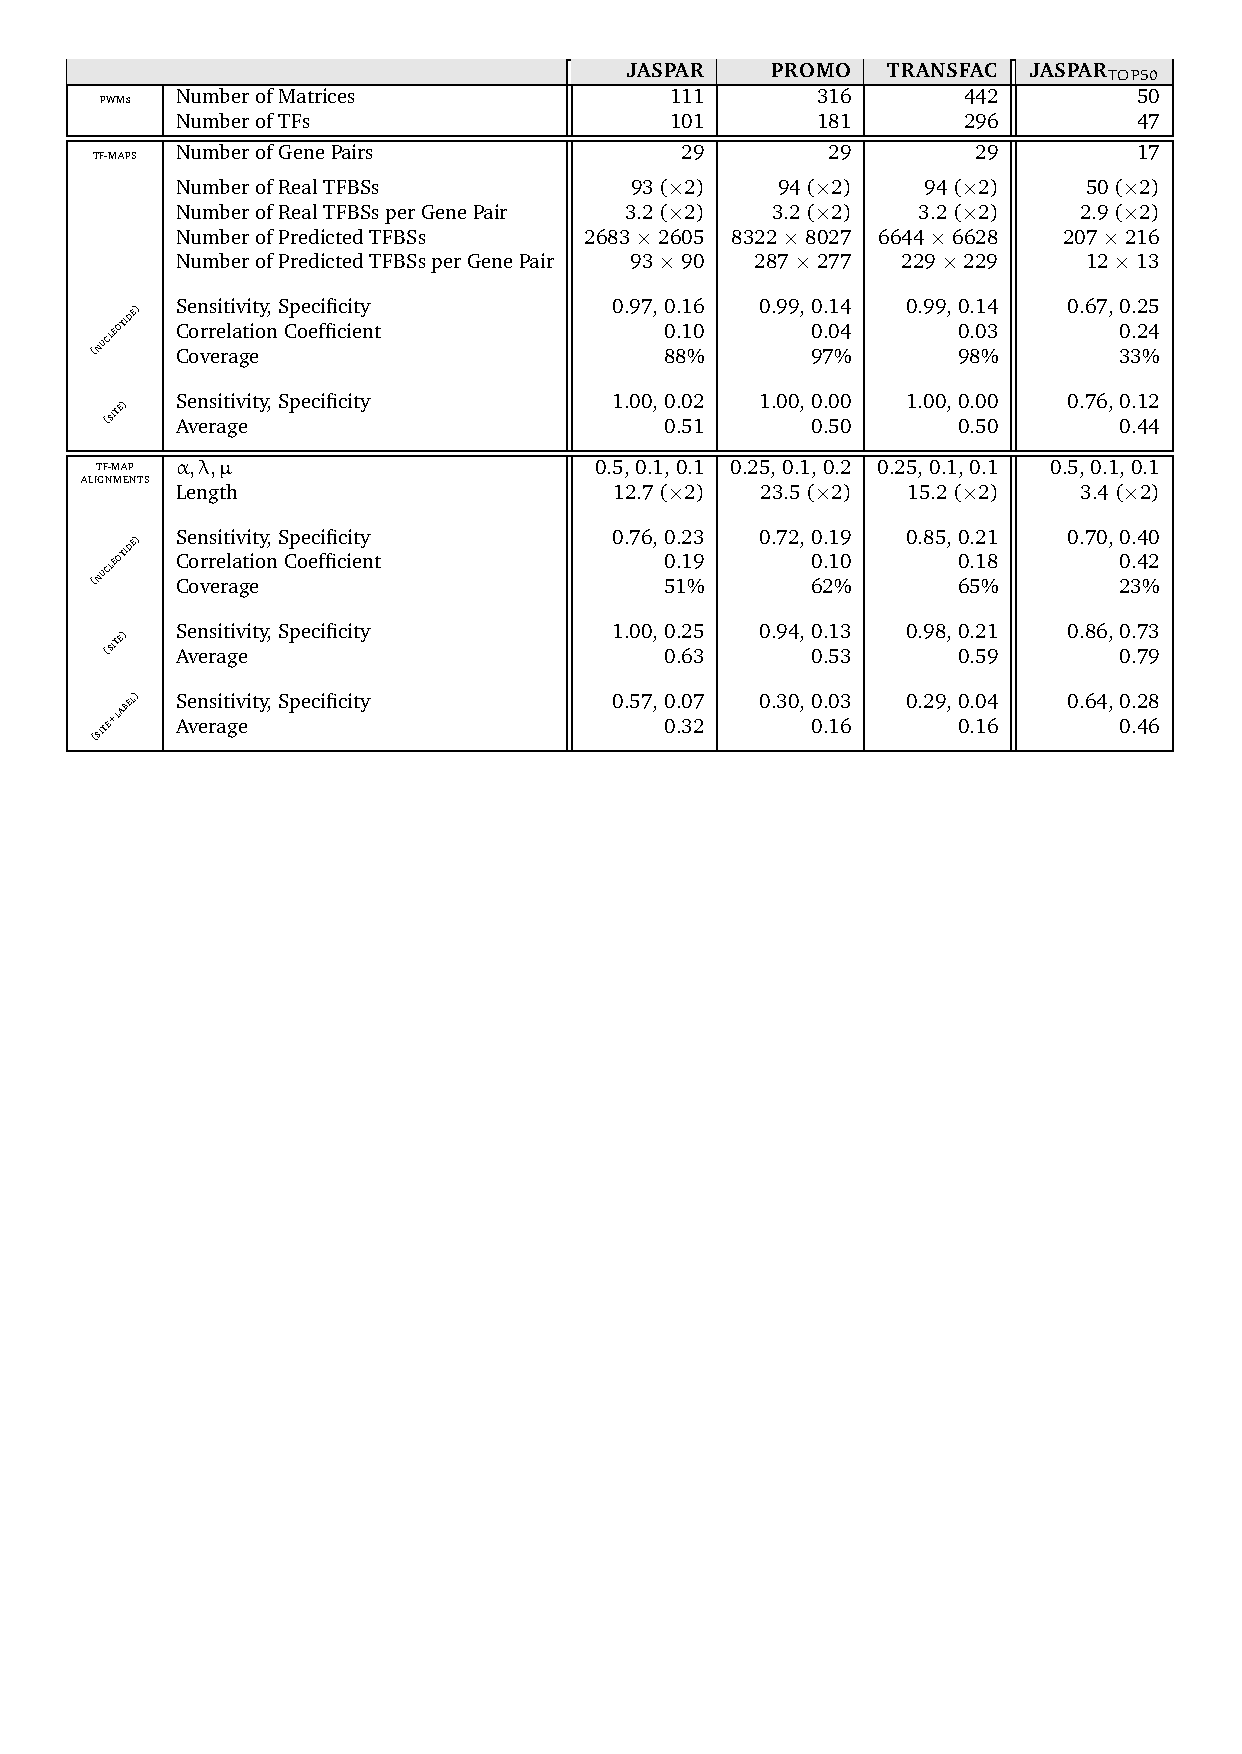
\includegraphics[bb=30 479 566 817,clip]{tables/maccuracy}
\end{center}
\end{minipage}
\mycaption{tab:accuracy}% label
          {TF-map alignment accuracy results on the \textsc{HR set}}% lof
          {TF-map alignment accuracy results on the \textsc{HR set}.}% caption header
          {\tiny Parameters were estimated independently using three
           different collections of  position weight matrices (PWMs) for
           transcription factor binding sites (TFBSs) to obtain the TF-maps of the
           promoter sequences. 
           The table has three parts. 
           On {\bf top},  number of matrices in each of these collections, and 
           the number of transcription factors (TFs) these matrices correspond to. 
           In the {\bf middle}, statistics of the resulting TF-maps: 
           number of promoter pairs (out of 36) for which matches to at least one 
           common TFBS was found in both the human and mouse orthologs 
           (and for which, therefore, there exist a non-void TF-map alignment), 
           total and average number of 
           real TFBSs per promoter sequence, total and average number of 
           predicted TFBSs per promoter sequence, and sensitivity and specificity 
           at the nucleotide and site levels (see main text for definitions). The 
           average sensitivity and specificity at the site level is the optimization 
           measure when estimating the parameters of the algorithm. Coverage is 
           the fraction of the sequence of the promoters covered by matches to TFBSs.
           At the {\bf bottom}, results of the optimal TF-alignments:
           optimal parameters and average length (number of aligned elements in the 
           optimal TF-map alignments), measures of sensitivity and specificity at the
           levels of nucleotide, site overlap, and site plus label match (see main 
           text for definitions). Coverage is the fraction of the sequence of the 
           promoters covered by matches to TFBSs.}
\end{center}
\end{table}
\end{landscape}

This number over the
total number of nucleotides in annotated TFBSs is the sensitivity, and over 
the total number of nucleotides in predicted TFBSs is the
specificity. Finally, as a summary of these two numbers we compute the
correlation coefficient. All the accuracy measures were also computed on
the initial PWM predictions, prior to the alignments.  

%%%%
% Figure 8: ABS
%%%%
\begin{figure}[t!]
\begin{center}
\setlength{\fboxsep}{0pt}
\fbox{\incgraph{width=0.85\linewidth}{ps/abs}}
\mycaption{fig:absweb}% label
          {Examples of the ABS data retrieval system}% lof
          {Examples of the ABS data retrieval system.}% caption header
          {The annotation of a gene, the set of binding motifs from a given TF in human 
           and mouse and the extraction of the promoter sequences containing such annotations
           \citep{blanco:2006a}.}% caption header.}
\end{center}
\end{figure}

\subsectionblue{Accuracy results}

\index{TF-map alignments!acc@accuracy} \index{meta-alignments!macc@accuracy} 
As it is possible to see, the main effect of the meta-alignment is the
dramatic reduction in the number of predicted TFBSs that typically
result after a PWM-based search (see also Figure \ref{fig:pspla}). Taking, for 
instance, the popular \db{Transfac} collection, the average number of TFBSs 
predicted per promoter in our dataset using this database is about 230. 
The TF-map alignment reduces this number approximately 15-fold, while 
the predicted TFBSs still covering essentially all annotated TFBSs \citep{blanco:2006b}. 
This gain in specificity is not simply due to the selection of an 
arbitrary set of non-overlapping TFBSs, since as a result of the map 
alignments the proportion of the promoter region covered by predicted 
TFBSs drops from 98\% to 65\% --a number which is more consistent with 
the estimated occupancy by TFs of the core promoter regions \citep{wray:2003a}. 

In this regard, we have compared the map alignments here with direct
sequence alignments in their ability to identify TFBSs in the promoter
regions of co-regulated genes. We have used NCBI-BLASTN \citep{altschul:1990a} 
to identify conserved blocks in the promoter region of the orthologous pairs in
the \textsc{HR set}. We have searched for local, instead of global
alignments because we expect the TFBSs to distribute discretely along
the promoter region --resulting in a patch of conserved and
non-conserved fragments. In addition, local alignments are insensible
to the relative rearrangements in the order of the TFBSs between the
promoters sequences compared. This is an advantage over the map
alignments, which require colinearity of the TFBSs in the sequences to
be compared. Despite this, and the fact that promoter elements are
usually embedded within well conserved sequences in human and mouse
orthologous promoters, map alignments are comparable or outperform the
BLASTN comparison when identifying TFBSs in them \citep{blanco:2006b}. The correlation
coefficient between the sequences covered by the BLASTN alignments and
the annotated TFBSs is $0.15$, while the same measure when considering
the sequences covered by the map alignments is $0.19$ for \db{Jaspar},
$0.10$ for \db{Promo} and $0.18$ for \db{Transfac}. Table \ref{tab:accuracy2} lists 
these values, as well as the the values of sensitivity and specificity. To obtain
these values, BLASTN was run with default parameters, but decreasing
the word size to 7 (the minimum accepted value in
NCBI-BLASTN). This allows for the detection of shorter and weaker
alignments. The performance of BLASTN degrades if we increase the word
size. We obtained similar results using the
WU-BLASTN version, which allows for shorter word sizes (data not shown).

%%%%%%%%%%%%%%%
%%% TABLE 2
%%%%%%%%%%%%%%%
\begin{table}[t!]
\begin{center}
\begin{minipage}{0.95\linewidth}\setlength{\parindent}{0pt}
\begin{center}
\scalebox{0.75}{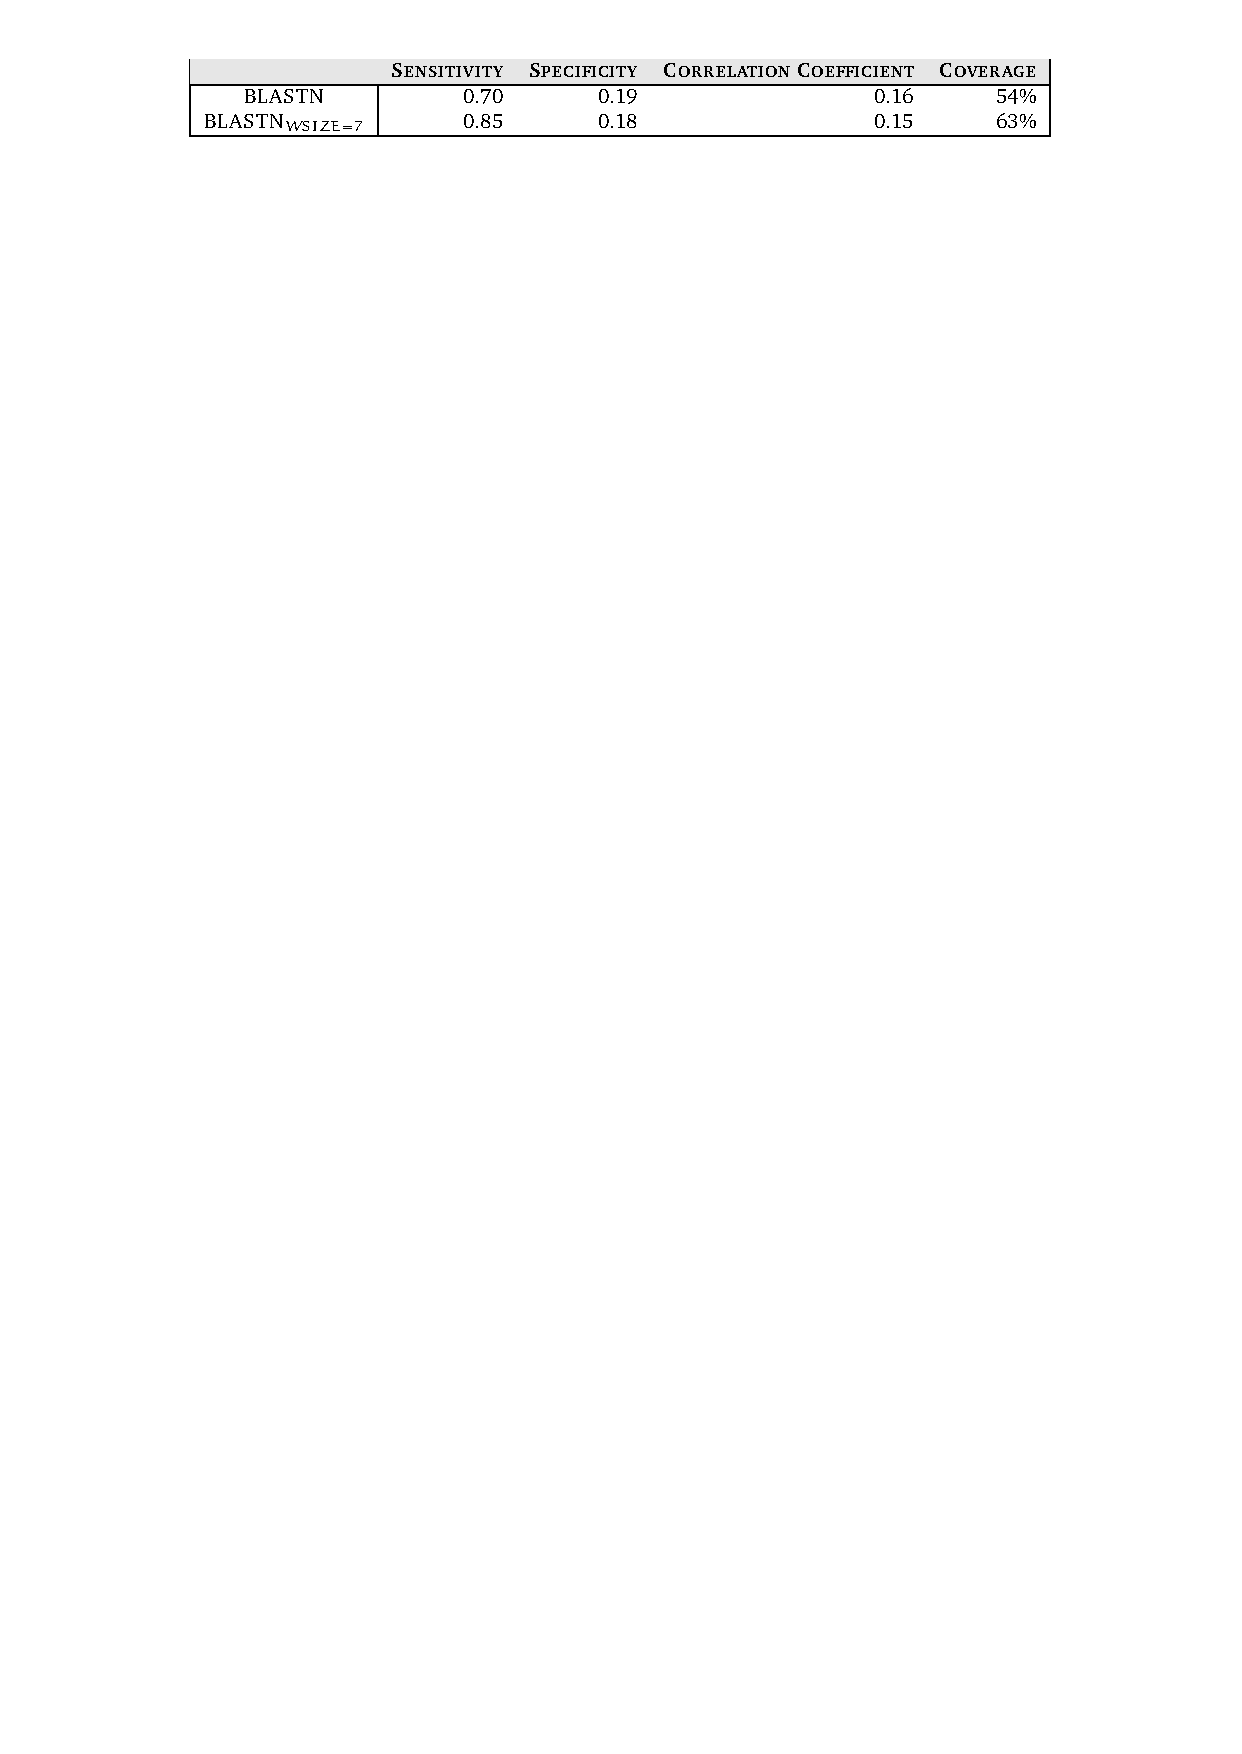
\includegraphics[bb=89 775 505 816,clip]{tables/maccuracy2}}
\end{center}
\end{minipage}
\mycaption{tab:accuracy2}% label
          {BLASTN accuracy results on the \textsc{HR set}}% lof
          {Results when using BLASTN to detect 
           conservation between orthologous pairs.}% caption header
          {}
\end{center}
\end{table}

The values in Table \ref{tab:accuracy} reflect differences between the three
collections of matrices when used in the context of the map
alignments. In this context, \db{Jaspar} appears to show the better balance
between sensitivity and specificity. This can be partially explained 
because there is less matrix redundancy --which in turn implies less
overprediction-- in \db{Jaspar} than in the other collections. To further 
minimize overprediction, we have computed the information content of 
all \db{Jaspar} matrices and selected the most informative ones. Let $P$ be 
a PWM where $P(x,i)$ denotes the probability of observing the  
nucleotide $x$ in the position $i$ of a motif of length $n$. The amount
of information $R$ of the matrix $P$ is defined as \citet{schneider:1990a}:

\begin{center}
\fcolorbox{white}{verylightgreen}{
\begin{minipage}[][][c]{0.95\linewidth}
\begin{equation}
R(P) = \sum_{i = 1 \ldots n} \left( 2 + \sum_{x\in A,C,G,T}{P(x,i) \log{P(x,i)}} \right).
\end{equation}
\end{minipage}}
\end{center}

When using the collection of the 50 \db{Jaspar} matrices with the highest $R$ value 
(which we refer to as \db{Jaspar$_{TOP50}$}) \index{JASPAR$_{TOP50}$}
to obtain the TF-maps, detection 
of TFBSs through map alignments improves over the entire set of \db{Jaspar} 
matrices: while there is some loss of sensitivity, there is a larger gain 
in specificity (see Table \ref{tab:accuracy}). 

%%%%
% Figure 9: PS-PLA1
%%%%
\begin{figure}[t!]
\begin{center}
\setlength{\fboxsep}{0pt}
\fbox{\incgraph{width=0.85\linewidth}{ps/pspla}}
\mycaption{fig:pspla}% label
          {TF-map alignment of the human and mouse PLA1A gene}% lof
          {TF-map alignment of the human and mouse PLA1A gene.}% caption header
          {Results of the TF-alignment of the human and mouse promoters of the 
           \emph{phospholipase A1 member A} gene (PLA1A, RefSeq entries NM\_015900, 
           NM\_134102). Here, the 2000 nucleotides upstream of the annotated 
           transcription start 
           site (TSS) have been considered (with position 1 corresponding to -2000). The
           TF-maps on these sequences were obtained using \db{Transfac} 6.3
           \citep{matys:2003a}. These maps contained 676 predicted binding 
           sites in human and  595 in mouse (threshold 85\%), and they are 
           represented graphically on the top right of the
           figure. Each box represents a different binding site and the color
           corresponds to the associated transcription factor (TF). The resulting
           TF-map alignment is also represented graphically at the bottom
           right. As it is possible to see, while the region 
           proximal to the TSS is not more dense in predicted TFBSs than other regions, 
           most of the aligned elements cluster near to the TSS. Indeed, more than 
           half of the elements in the TF-map alignments are within 500 nucleotides of the TSS. 
           The program GFF2PS \citep{abril:2000a} has been used to obtain the graphical 
           representation of input predictions and final alignment.}
\end{center}
\end{figure}

Finally, we have also performed a complementary
test to measure the specificity of the TF-map alignments \citep{blanco:2006b}. 
As a negative control, we have shuffled the orthologous pairing in the
\textsc{HR set} to construct a pool of unrelated human-mouse gene pairs. 
Then, the corresponding TF-map alignments between these non-orthologous paired
promoters were obtained using the parameters previously optimized.
For the three collections of matrices, the  TF-map alignments
between pairs of unrelated promoters were significantly shorter with
an average score about 50\% smaller than TF-map alignments between
``bona fide'' orthologous promoters. For instance, the average length of 
the TF-map alignments between orthologous promoters when using the \db{Jaspar} 
collection was 12.7 TFBSs, with an average score of 55.2. In contrast, 
the length of the TF-map alignments between non-related promoters was 
8.36 TFBSs, with an average score of 20.67. The sites in the
alignments involving non-orthologous gene promoters may hypothetically
correspond to general regulatory elements present in most
core promoters. An alternative, more probable, hypothesis is that they
reflect the poor specificity of most PWMs representing TFBSs.
Indeed, when we perform the same test using the more
informative \db{Jaspar}$_{TOP50}$ collection, no TF-map alignments can be 
obtained between any pair of the non-related promoters.

\sectiongreen[TF-map alignments in orthologous genes]{Using TF-map alignments to distinguish promoters from other genomic regions} 
\label{sec:testregions}

Results in the previous section indicate that alignments of TF-maps
can contribute --together with other tools, such as primary sequence
alignments-- to the characterization of the promoter region of
co-regulated genes. This contribution is mostly 
obtained through the substantial reduction of the overwhelming number 
of candidate TFBSs that PWMs and other pattern based searches 
typically produce. The co-regulated genes in the test 
case of the previous section, however, were orthologous human-mouse
pairs. The promoter regions of such pairs show substantial sequence 
conservation \citep{waterston:2002a}. It can be argued that under such 
circumstances map alignments may not be much more informative than 
primary sequence alignments. Note that, in general, good alignments 
at the primary sequence level will inevitably result 
--given the low specificity of the PWM search-- in good 
map alignments, although such map alignments may bear 
little relationship to the underlying conserved 
configurations of TFBSs. To assess to what extent good 
TF-map alignments are simply a reflection of underlying 
sequence conservation, we have compared the meta-alignments obtained using 
\db{Jaspar}$_{TOP50}$, in the 200 nucleotides of the promoter region of the 36 
gene pairs from the \textsc{HR set}, with the meta-alignments obtained in fragments 
of 200 nucleotides from intergenic (2000 nucleotides upstream of the TSS), 
5'UTR (downstream of the TSS), coding (downstream of the translation start 
site and considering only coding DNA), intronic (downstream of the first intron 
junction), and downstream (downstream of the transcription termination 
site) sequences. The test is graphically represented In Figure 
\ref{fig:testregions}.

We have computed the average score of the map alignments in each of the genomic 
regions and have identified, for each homologous pair, the genome regions in which 
the alignment produces the highest score \citep{blanco:2006b}. We have performed 
the same exercise using global pairwise sequence alignments, obtained with CLUSTALW 
\citep{thompson:1994a}. 
Results appear in Table \ref{tab:testregions} (Top). As expected, nucleotide sequence
alignments score the highest in the coding regions (in 26 out of 36
cases), followed by the alignments in the promoter (5 out of 36) and
5$^\prime$ UTR regions (4 out of 36). The scores of the sequence 
alignments show that promoter regions are less conserved than coding regions,
and have a level of conservation similar to that observed in 5'UTRs. 
Despite this, TF-map alignments score the highest in the promoter
regions (in 25 out of 36), where the average score of map alignments 
is almost twice as high as that of the coding regions. Only in 6 out
of 36 cases the TF-map alignment scores the highest in coding regions. 
Interestingly, while intron sequences in the orthologous human-mouse
pairs are much less conserved than 5'UTRs, TF-map alignments 
have a similar score in both regions. In fact, in 3 cases, TF-map
alignments have the highest score in first introns, while only in 1 case in
5'UTRs. This is consistent with the fact that first introns are known
to often contain regulatory motifs. 

%%%%
% Figure 10: TestRegions
%%%%
\begin{figure}[t!]
\begin{center}
\setlength{\fboxsep}{0pt}
\fbox{\incgraph{width=0.75\linewidth}{ps/testregionsS}}
\mycaption{fig:testregions}% label
          {TF-map alignment on several genomic samples}% lof
          {TF-map alignment on several genomic samples of two species.}% caption header
          {}
\end{center}
\end{figure}

In order to measure the ability of TF-map alignments
to detect conserved regulatory elements at larger
evolutionary distances --at which the degree of sequence
conservation may be negligible-- we have carried out the same analysis
on a set of human-chicken orthologous pairs derived from the \textsc{HR
set}.  Using the RefSeq gene set as mapped into the UCSC genome browser,
we have identified the chicken ortholog for 25 genes in the
\textsc{HR set}. We refer to the resulting set of human-chicken gene pairs as the
\textsc{HC set} \citep{blanco:2006b}. As before, we have compared
promoter, intergenic, 5'UTR, coding, intronic and downstream sequences
between the orthologous human-chicken genes using both TF-map
alignments based on \db{Jaspar}$_{TOP50}$ and sequence alignments using CLUSTALW.
Results appear in Table \ref{tab:testregions} (Bottom). 
While, as expected, the scores of the alignments are, in both cases, clearly
lower for human--chicken than for human--mouse comparisons,
the same relative trends can be observed, with sequence alignments
being most significant between coding regions, and TF-map alignments
between promoter regions.
However, while coding sequences are still distinctively conserved
between human and chicken, similarity in promoter sequences degrades
substantially.  
Indeed, in contrast with human-rodent comparisons,  5'UTRs are, for
instance clearly more conserved than the promoters between human and chicken
orthologous genes. Despite this lack of sequence similarity in the
human-chicken promoter pairs and the fact that we trained our
algorithm specifically on human and rodent genes, 
the TF-maps remarkably still score the highest in these regions (in 9 out of 25).
Interestingly, TF-map alignments are able to score comparatively high 
in downstream regions even though they do not appear to exhibit
sequence conservation; regulatory
motifs have been occasionally reported on these regions.
Overall, these results indicate that alignments of TF-maps are able to detect
conservation of regulatory signals, which can not be detected by
sequence similarity alone \citep{blanco:2006b}.

%%%%%%%%%%%%%%%
%%% TABLE 3
%%%%%%%%%%%%%%%
\begin{table}[t!]
\begin{center}
\begin{minipage}{0.98\linewidth}\setlength{\parindent}{0pt}
\begin{center}
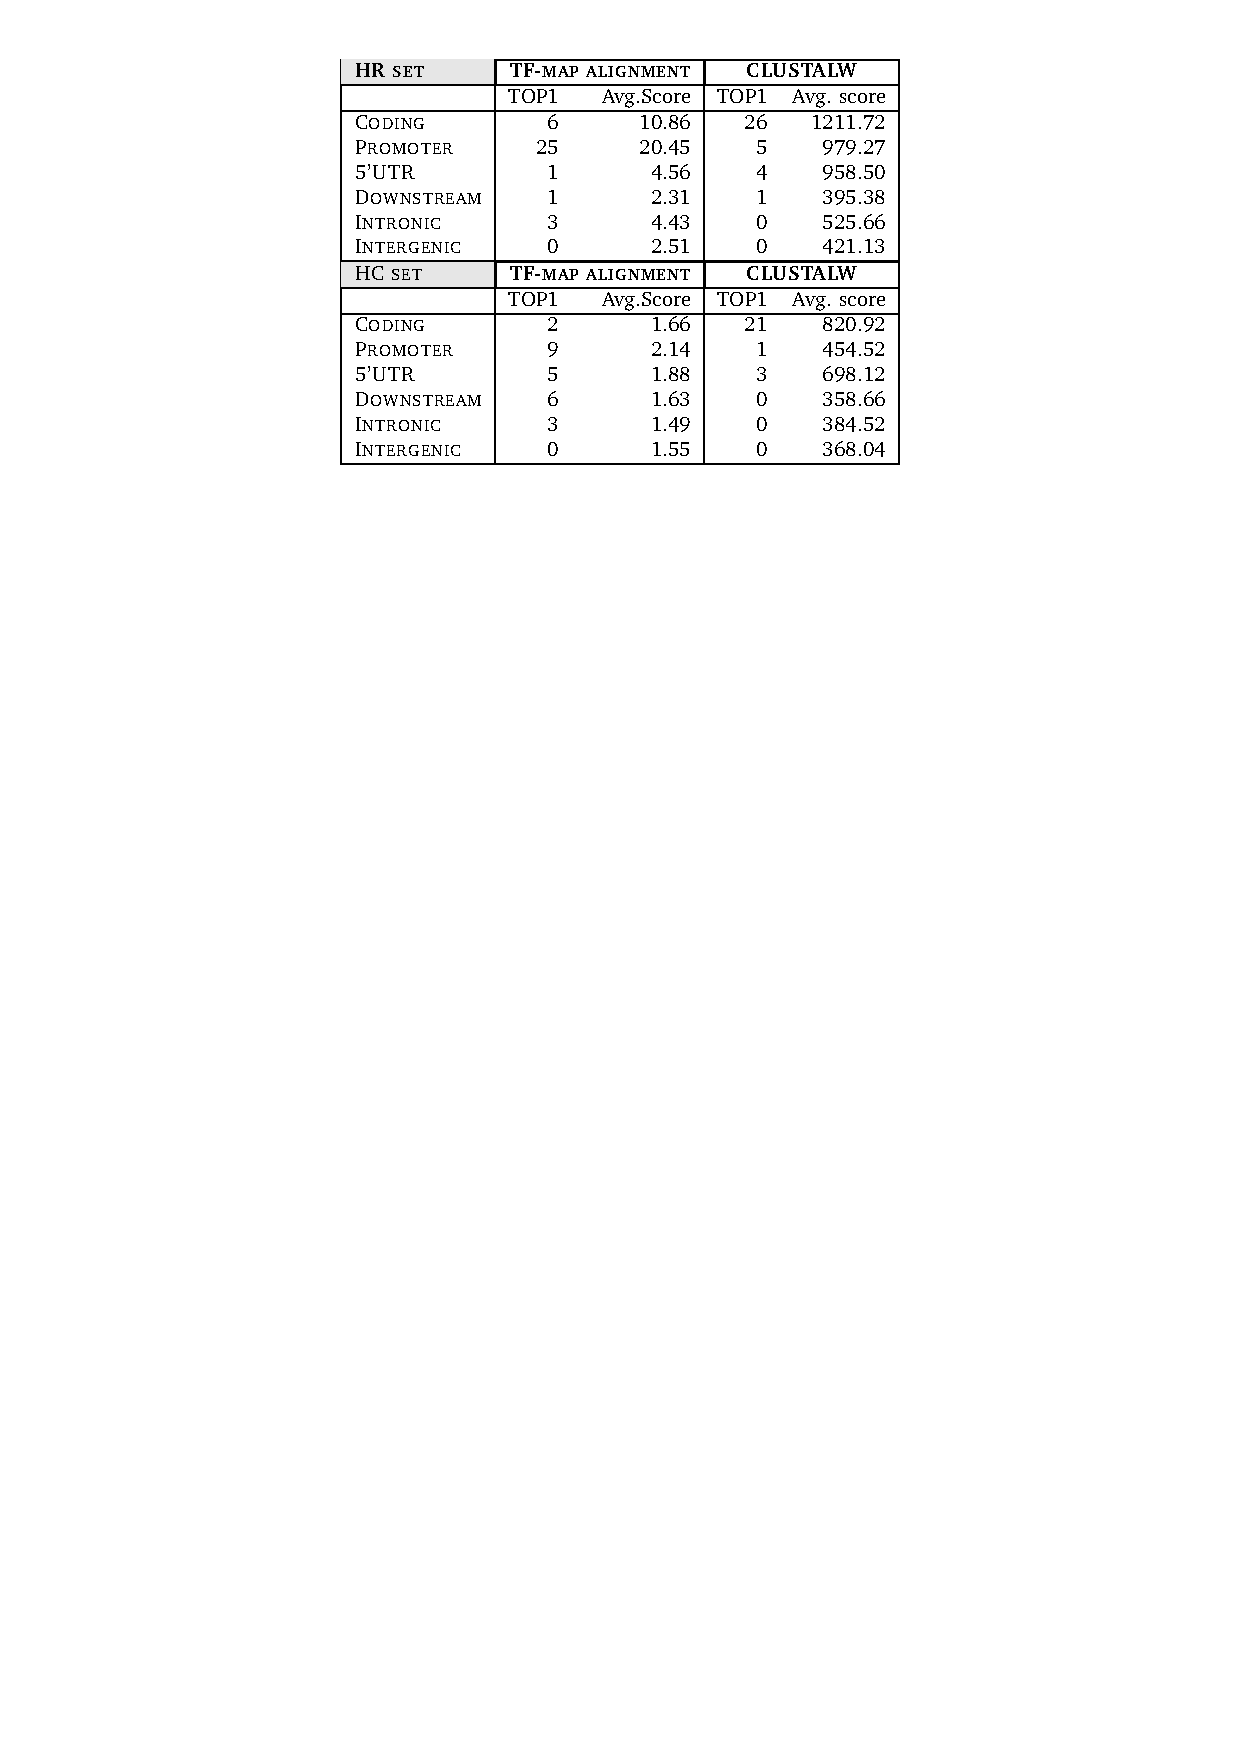
\includegraphics[bb=161 608 434 816,clip]{tables/testregions}
\end{center}
\end{minipage}
\mycaption{tab:testregions}% label
          {TF-map alignment results on several genomic samples.}% lof
          {TF-map alignment results on several orthologous genomic samples}% caption header
          {(Top) Sequence and TF-map alignments of different genomic regions
           between the human and mouse orthologous pairs in the \textsc{HR set}. 
           (Bottom) Sequence and TF-map alignments of different genomic regions
           between the human and chicken orthologous pairs in the \textsc{HC set}.
           TOP1 is the number of pairs in which the highest scoring alignment is found 
           in a given genomic region.}
\end{center}
\end{table}

\subsectionblue{Promoter identification with TF-map alignments}

\index{TF-map alignments!prom@promoter identification} \index{promoter!idtf@identification} 
Promoter identification is still a difficult problem (reviewed in Chapter 
\ref{sec:genefinding}). TF-map alignments may be helpful in this problem. Using a set
of $278$ orthologous human-chicken gene pairs of another study \citep{abril:2005a},
we have performed the following experiment.

We have extracted the human promoter of these genes ($500$ nucleotides) from the 
UCSC human genome distribution according to the RefSeq coordinates. For the chicken 
genes, we have extracted the mRNA from the chicken genome surrounded by $5,000$ 
nucleotides upstream of the TSS and $5,000$ downstream of the end of the transcript. 
Finally, we have extracted samples of $500$ nucleotides from these long sequences,
without overlapping between each contiguous windows. For each gene, the upstream promoter 
region, orthologous to that of human, is therefore located in the window between the 
positions $4,500$ and $5,000$ nucleotides (see Figure \ref{fig:testpromoterpgws}).

Next, we have used the $50$ more informative matrices from \db{Transfac} \citep{matys:2003a} 
as a mapping function to obtain the
map of each sample in the chicken sequences. We have also used \db{Transfac} for mapping
the predicted TFBSs on the human promoters. The experiment consisted in
performing the pairwise TF-map alignment between the human promoter and all of the
samples in its chicken ortholog. Then, for each window we have counted in how many
cases out of the $278$ genes the TF-map alignment between the human promoter and that 
window sample scores the highest, among all of the windows. As shown in Table 
\ref{tab:testpromoter}, the chicken gene fragment in which more genes hit the best 
was the $4,500-5,000$ sample (31\%), which corresponds with the upstream promoter region 
according to the RefSeq annotations. In addition, 14\% and 21\% of the 278 gene pairs 
obtained the highest TF-map alignment score on the windows located at $4,000-4,500$ and 
$5,000-5,500$, respectively. This bias is not observed in the rest of the windows.
These percentages agree well with the errors in the precise TSS annotation \citep{suzuki:2004a}.

We also counted for each window in how many cases the meta-alignment between this
sample and the human orthologous promoter scores among the TOP-10 best alignments.
Despite the results are less significant, it is interesting to notice that in more
than 200 gene pairs (76\%), the TF-map alignment between the human promoter and
the chicken sample in the window $4,500-5,000$ was among the TOP-10.
We repeated the test with the full collection of \db{Transfac} 6.3 ($442$ matrices). The
results, shown in Table \ref{tab:testpromoter}, are slightly worse. This fact is
probably related to the poor specificity of many matrices that are included in the full 
collection.

Again, we performed the same experiment with the program BLASTN, using the score of the 
best HSP on each alignment to rank the window comparisons. Table \ref{tab:testpromoter} 
lists the results. The sequence alignments can detect correctly the actual promoter 
pair in less than 16\% of the $278$ genes (31\% among the best 10 alignments).

Future experiments should be conducted in a genome-wide mode to verify the accuracy
of TF-map alignments in larger datasets. However, the meta-alignment, at least in this 
set of $278$ gene pairs, was clearly superior to sequence alignment to detect the correct
promoter region. In principle, we could be able with the TF-map alignments 
to accurately detect the promoter region in one species, scanning this genome with the 
orthologous promoter in the other informant genome.

%%%%
% Figure 11: testPromoterRegion
%%%%
\begin{figure}[t!]
\begin{center}
\setlength{\fboxsep}{0pt}
\fbox{\incgraph{width=0.75\linewidth}{ps/testpromoter}}
\mycaption{fig:testpromoterpgws}% label
          {TF-map alignment in promoter detection}% lof
          {TF-map alignment in promoter detection.}% caption header
          {}
\end{center}
\end{figure}

\subsubsectionblue{Parallel meta-alignment: PGWS}
\index{meta-alignments!pgws@parallel} \index{PGWS}
Let $M$ be a long genomic region of $m$ nucleotides. Let $P$ be a short genomic 
sequence of $p$ nucleotides, with $m >> p$. The problem of mapping and aligning 
the sequence $P$ to a contiguous set of windows in $M$ must be carefully analyzed
to obtain in a reasonable  amount of time that window from $M$ whose TF-map alignment 
to $P$ reaches the highest value. If $p=500$ bps, $m=20,000$ bps and the windows are 
$500$ bps with an overlap between adjacent windows of $100$ bps then the number of 
windows (that matches the number of pairwise TF-map alignments to do) is 50. Obviously, 
if the test is repeated for hundreds of gene pairs, the computation of the best windows 
requires some improvement.

In fact, the calculation of the TF-map alignment between $P$ and a given window from
$M$ is independent from the rest of alignments. Thus, the alignments can be easily
dispatched to different processors to be performed in parallel. At the end of the
process, the scores of the alignments are ranked and displayed. Notice we are only 
interested in the score of the alignments to construct a ranking so the TFBSs that 
actually constitute them are logically not necessary in this case. Thus, we
register the value calculated on each dynamic programming similarity matrix,
but the paths of the alignments are not constructed.

Following with the same example: if there are $10$ available processors, we can divide
uniformly the list of windows (alignments) among them using any offset schema to
ensure the load of each processor is similar. For instance, if we consider an
offset of $4,000$ bps between two windows that are processed by the same unit,
we will assign the series of alignments 
$(M_{0-500},M_{4000-4500},M_{8000-8500},M_{12000-12500},M_{16000-16500}$
to the processor $P_1$, the series 
$(M_{400-900},M_{4400-4900},M_{8400-8900},M_{12400-12900},M_{16400-16900}$
to the processor $P_2$ and so on. The chronograph of events associated to
this parallel processing is:

\begin{center}
\setlength{\fboxsep}{0pt}
\incgraph{width=0.75\linewidth}{ps/chronogram}
\end{center}

In this case, we can divide the sequential time $T(n)$ by the number of
processors so that the parallel time is $\frac{T(n)}{10}$. We can then
compute $50$ TF-map alignments with $10$ computers using the same amount
of time that is necessary for calculating $5$ alignments in a single processor
machine. As the same comparisons must be done for hundreds of genes, the
save of time using this parallel version is considerable. 

The program \prog{pgws} (Promoter Genome-Wide Search) is a generalization of
the schema presented here, in which the input consists of a list of probes
$P=p_1,p_2 \ldots p_{|P|}$ (gene promoters from species $A$) and a list of long
genomic sequences $M=m_1,m_2 \ldots m_{|M|}$ (chromosomes from species $B$).
In an efficient parallel environment, the program \prog{pgws} may be used, for 
instance, to locate the ortholog promoter of a chicken gene in the human genome.


\sectiongreen[TF-map alignments in co-regulated genes]{Using TF-map alignments to characterize promoter regions of 
co-regulated genes}\label{sec:cisred}

\index{TF-map alignments!cisred@in CISRED} \index{meta-alignments!mcisred@in CISRED} 
We expect, therefore, the map alignments to be particularly useful to
characterize promoter regions of co-regulated genes in absence of
sequence conservation. In such cases, the map alignments can help to
recover conserved configurations of TFBSs that primary sequence
comparisons would not. It is important to stress in this regard, that
the match state in the alignment of TF-maps is defined based on the
transcription factor label, and not based on the label of the specific
binding site. Since a given TF can be associated to
different binding sites (for instance, the approximately 90 TFBSs in
the \textsc{HR set} correspond only to about 30 TFs), an alignment of TF-maps
can include the alignment of TFBSs that show no sequence conservation.

%%%%%%%%%%%%%%%
%%% TABLE 4
%%%%%%%%%%%%%%%
\begin{table}[t!]
\begin{center}
\begin{minipage}{0.98\linewidth}\setlength{\parindent}{0pt}
\begin{center}
\scalebox{0.8}{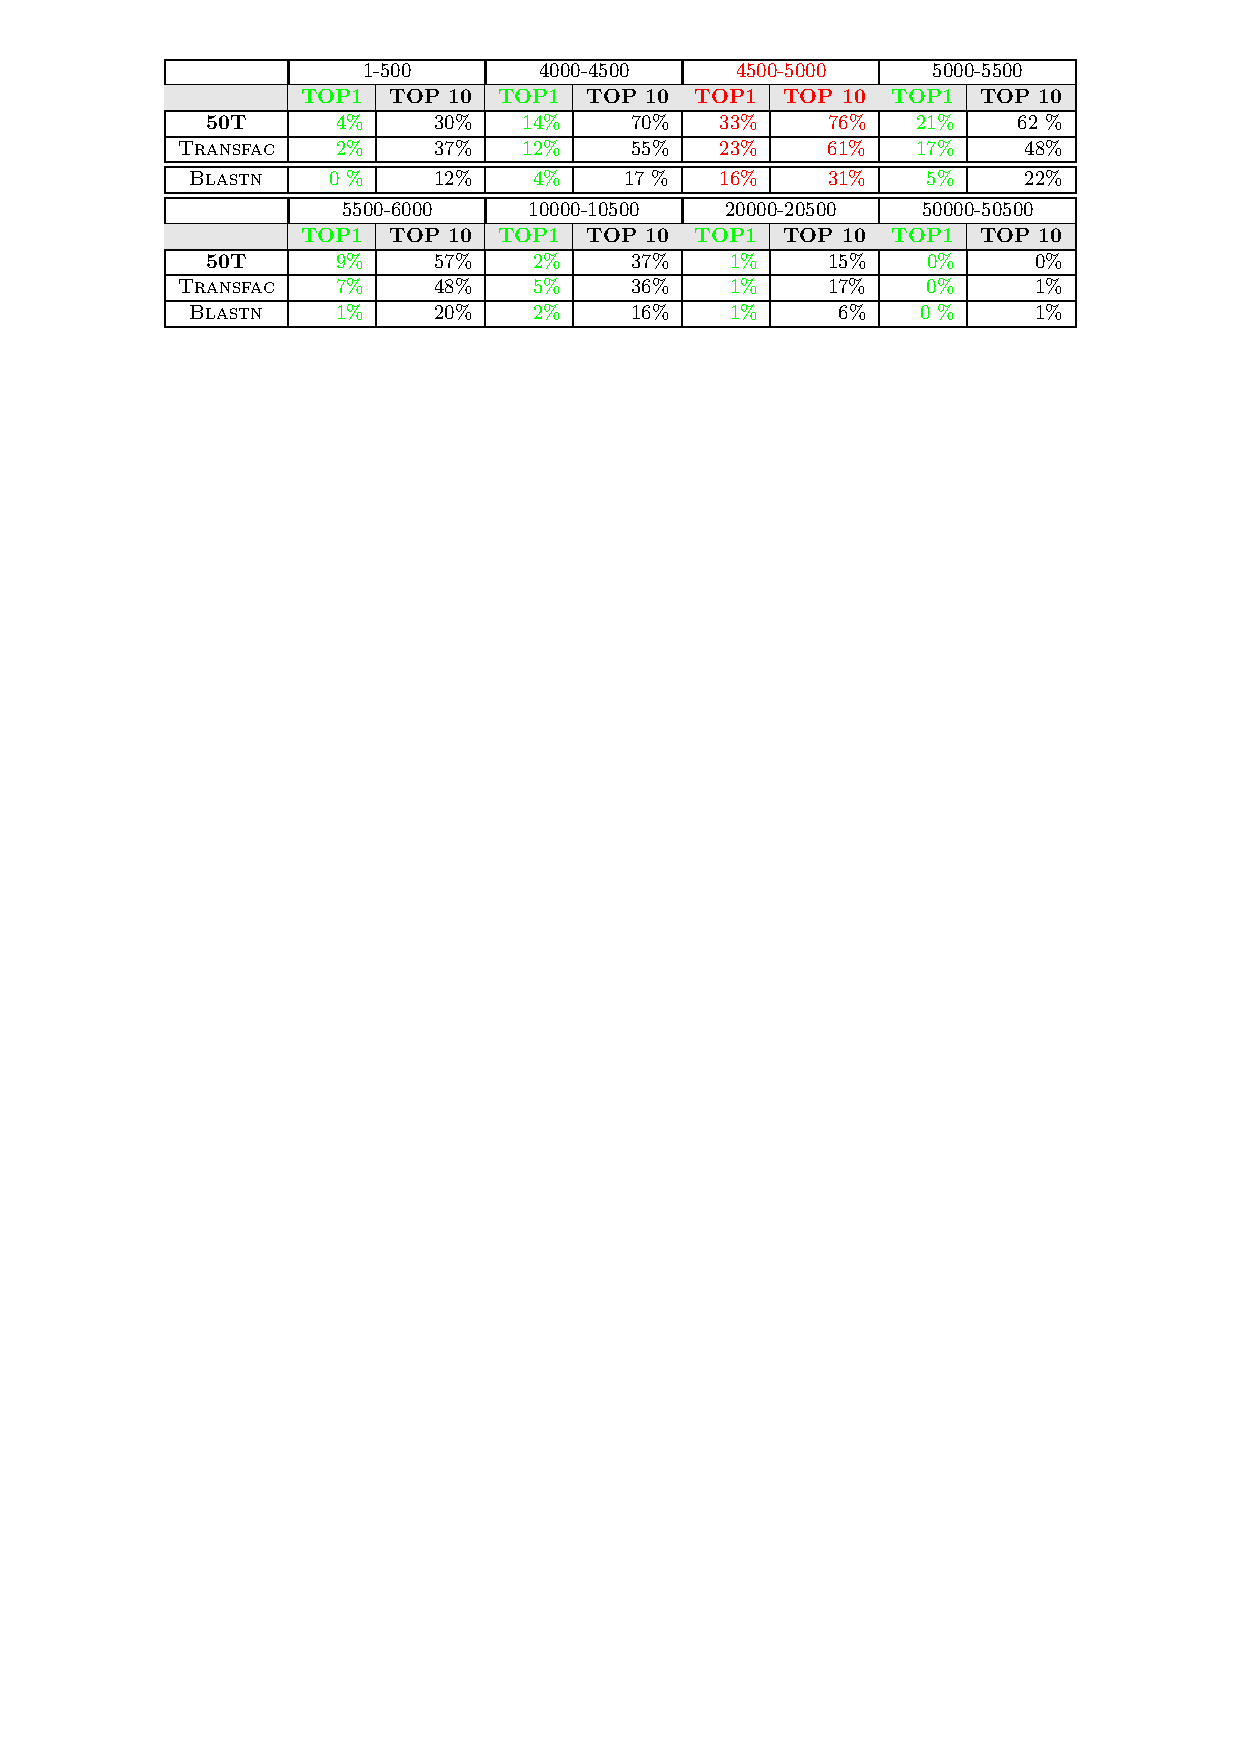
\includegraphics[bb=75 681 519 817,clip]{tables/testpromoter}}
\end{center}
\end{minipage}
\mycaption{tab:testpromoter}% label
          {Promoter identification with human-chicken TF-map alignments}% lof
          {Promoter identification with human-chicken TF-map alignments.}% caption header
          {The percentages are relative to the proportion of the $278$ human-chicken promoter
           pairs that score the highest in each window (or within the TOP 10). The correct 
           promoter window is $4,500-5,000$. The $50$T collection are the $50$ more informative 
           matrices from \db{Transfac}.}
\end{center}
\end{table}

Many examples could be found in which map alignments produce a better
characterization of the promoter region of co-regulated genes than
that obtained through primary sequence alignments. We would like,
however, to move beyond such an anecdotal evidence, and have a more
exhaustive evaluation of the power of TF-map alignments to characterize
promoter regions of co-regulated genes in absence of sequence
similarity. Towards such a goal we have used the set of co-regulated
genes in the CISRED database \citep{robertson:2006a}. The CISRED \index{CISRED}
database is primarily a collection of conserved regulatory sequence
elements identified by a genome-scale computational system that uses
pattern discovery, similarity, clustering, co-occurrence and co-expression 
calculations. CISRED includes, as well, a database of high-confidence 
co-expressed gene pairs \citep{griffith:2005a}, obtained from cDNA microarray 
hybridization, SAGE and other experiments, as well as Gene Ontology 
(GO, \cite{tgoc:2000a}) analysis. Version 1 of CISRED high confidence 
co-expression human set contains 60,912 co-expression gene pairs for 5562 genes. 
Because of the criteria to establish co-regulation within CISRED, we do not 
expect strong bias towards co-expression pairs sharing strong sequence 
similarity in their promoter regions. 

We have, thus,  performed the following experiment (graphically represented
in Figure \ref{fig:cisred}):
we have compared the promoter region of each gene $x$ in the CISRED
set with the promoter regions of the genes co-regulated with $x$,
$coreg(x)$, and with the promoter region of the genes no co-regulated
with $x$, $\overline{coreg}(x)$. Even though the promoter of the gene
$x$ may not show stronger sequence similarity with the promoters of the
genes in $coreg(x)$ than with the promoters of the genes in 
$\overline{coreg}(x)$, our assumption is that it will still share
some common regulatory signal (maybe very weak) with the promoters of
the (at least a fraction of) the genes in $coreg(x)$, whereas no
common signal will be shared between the promoter of $x$ and the
promoters of the genes in $\overline{coreg}(x)$. Our hypothesis is
therefore that alignments of TF-maps will be superior in detecting
such signals to alignments of the primary nucleotide sequence. 

We have proceed in the following way:
we have used ENSMART to extract 500 nucleotides
upstream of each gene in CISRED according to genome coordinates in 
\ensembl{}. We have used 500 nucleotides upstream here, instead of 
200 nucleotides as before, because of the intrinsic imprecision 
of \ensembl{} when annotating the coordinates of the TSS.  
We obtained such a sequence for 5333 out of 5562 CISRED genes
and considered it the promoter region of the gene. For this set of 
5333 genes, 56,632 co-expression gene pairs are described in CISRED.
We have used next the collection
of matrices in \db{Jaspar}$_{TOP50}$ (see previous section) to obtain the
TF-maps of each promoter region. Then for each gene
$x$ we have obtained the optimal map alignment with each gene in
$coreg(x)$ and in $\overline{coreg}(x)$. We have used the enhanced 
TF-map alignment algorithm
with the optimal parameters estimated in the training procedure. 
Finally, we have determined whether
the scores of the map alignments between the promoter of gene $x$ and
the promoters of the genes in $coreg(x)$ were significantly higher
than the scores of the map alignments between the promoter of gene $x$
and the promoters of the genes in $\overline{coreg}(x)$. Because the
scores of the optimal TF-maps alignments follow, as optimal sequence
\index{TF-map alignments!dis@score distribution} \index{meta-alignments!mdis@score distribution} 
alignments, a Gumbel or extreme-value distribution (see Figure \ref{fig:gumbel}), 
we calculated the Wilcoxon test to assess this
hypothesis. We obtained 42,756 non-void $coreg(x)$ alignments and 
20,600,640 non-void $\overline{coreg}(x)$ alignments. 
4,784 genes in CISRED had non-void alignments for both the 
$coreg(x)$ and the $\overline{coreg}(x)$ sets . The
average score of the $coreg(x)$ alignments was 6.02, and the average
length 2.13 sites. For the $\overline{coreg}(x)$ alignments, the values were
5.57 and 2.06, respectively. For 97 genes,
the score of the $coreg(x)$ alignments was significantly
higher than that of the $\overline{coreg}(x)$ alignments at a
significance level of p=0.01. At a p-value of 0.001, the number was 23. 
Since CISRED is partially based on microarray
experiments, one could argue that cross-hybridization with recently
duplicated genes may artefactually bias these results. However, no 
duplicated copies of genes exist in the sets of co-regulated genes with 
the 97 positive cases above.

%%%%
% Figure 12: the CISRED experiment
%%%%
\begin{figure}[t!]
\begin{center}
\setlength{\fboxsep}{0pt}
\fbox{\incgraph{width=0.75\linewidth}{ps/cisred}}
\mycaption{fig:cisred}% label
          {Alignment experiment with the CISRED genes}% lof
          {Alignment experiment with the CISRED genes.}% caption header
          {}
\end{center}
\end{figure}

We performed the same experiment, using BLASTN \citep{altschul:1990a} 
instead to compare the promoter region of each gene $x$ in the CISRED set 
with the promoters of the genes in $coreg(x)$ and $\overline{coreg}(x)$. 
BLASTN was used with the parameters word size 7 and expectation value 10 
so that short stretches of conservation could also be retrieved. In each 
comparison, we identified the score of the best HSP. We obtained 981 $coreg(x)$
alignments and 445,371 non-void $\overline{coreg}(x)$ alignments.
653 genes in CISRED had BLASTN alignments in both the 
$coreg(x)$ and the $\overline{coreg}(x)$ sets. The
average score of the $coreg(x)$ alignments was 29.9, and the average
length 51 nucleotides. For the $\overline{coreg}(x)$ alignments, the values 
were 24.3 and 40.5, respectively. For 11 genes,
the score of the $coreg(x)$ alignments was significantly
higher than that of the $\overline{coreg}(x)$ alignments at a
significance level of p=0.01;  there was
only one gene for which the score of the $coreg(x)$ alignments was 
significantly higher than that of the $\overline{coreg}(x)$ alignments,
at a significance level of p=0.001. 

We have investigated whether differences in conservation of regulatory
elements could be found between promoters associated to CpG islands
(CpG+) and promoters not associated to them (CpG-). CpG- promoters
have been linked to tissue-specific expression patterns 
\citep{smale:2003a}, and therefore they could be
overrepresented in the set of co-expressed genes for which we have
been able to identify conserved regulatory motifs. 
We computed for each gene the GC content and the CpG score as defined by
\citet{yamashita:2005a}. The presence of a CpG island on a window (-100:+100)
centered around the TSS of a gene is accepted when its GC content is
greater than 0.5 and when its CpG score is greater than 0.6 (CpG+); 
otherwise they are classified as CpG
negative genes (CpG-). Genes lacking CpG islands around their TSS have been
shown to have a more tissue-specific expression pattern
\citep{yamashita:2005a}. 
Based on these considerations, 3844 out of the 5333 promoters (72\%)
were identified as CpG+ genes, while only 1489 (28\%) were classified as
CpG-. Among the 97 genes for which  
the score of the $coreg(x)$ TF-map alignments was significantly
higher than that of the $\overline{coreg}(x)$ alignments at a
significance level of p=0.01, 63 were CpG+ (65\%). At a p-value of
0.001, the number of CpG+ genes was 13, out of a total of 23 (56\%).
It, thus, indeed appears that genes with CpG- promoters are slightly
overrepresented in the set of co-regulated genes with conserved
(specific) regulatory signals.

%%%%
% Figure 13: gumbel distributions
%%%%
\begin{figure}[t!]
\begin{center}
\setlength{\fboxsep}{0pt}
\begin{tabular}{|cc|}
\hline
\incgraph{width=0.35\linewidth,height=8cm}{ps/gumbel1} &
\incgraph{width=0.35\linewidth,height=8cm}{ps/gumbel2}\\
\hline
\end{tabular}
\mycaption{fig:gumbel}% label
          {Score distribution of the CISRED TF-map alignments}% lof
          {Score distribution of the CISRED TF-map alignments.}% caption header
          {(Left) Distribution of the $coreg(x)$ TF-map alignment scores. 
           (Right) Distribution of the $\overline{coreg}(x)$ TF-map alignment scores.}
\end{center}
\end{figure}


As it is possible to see, despite the general poor ability of both the
sequence alignments and the TF-maps to uncover relationships between
the promoters of the co-regulated genes in CISRED, it is clear that
TF-map alignments are able to detect more relationships than
BLASTN alignments (97 vs. 11 at a  p-value $<$ 0.01, 23 vs. 1 at a
p-value $<$ 0.001). It can be argued that this is partially an artefact,
resulting from BLASTN reporting only sequence alignments over a given
threshold, while non void TF-map alignments are always produced, provided that
the maps to align share at least one common element. 
In fact, given the number of genes for which valid alignments are
obtained, at a p-value $<$ 0.01 there are twice as many cases in 
which $coreg(x)$ scores are significantly higher than $\overline{coreg}(x)$ as 
expected if there was actually no difference in the distributions of scores, both using 
TF-map and sequence alignments.
At a p-value $<$ 0.001, however, the number of cases in which $coreg(x)$ scores
are significantly higher than $\overline{coreg}(x)$ coincides with the expected 
value using BLASTN, but it is five times the expected value, using TF-maps. 
We believe that this indicates that, even after taking into account the
effect of the different number of total alignments reported, 
the TF-map alignment algorithm is superior to BLASTN in
detecting relationships between the promoter regions of co-regulated
genes. Indeed, among the 445,371 total BLASTN alignments obtained,
there are 981 alignments between co-regulated genes, while 
the 445,371 top scoring TF-map alignments obtained include 1240
alignments between co-regulated genes.
Interestingly, there are only 148 alignments in common
between both approaches, indicating that they could be used to
complement each other.

%%%%%%%%%%%%%%%
%%% TABLE 5
%%%%%%%%%%%%%%%
\begin{table}[t!]
\begin{center}
\begin{minipage}{0.98\linewidth}\setlength{\parindent}{0pt}
\begin{center}
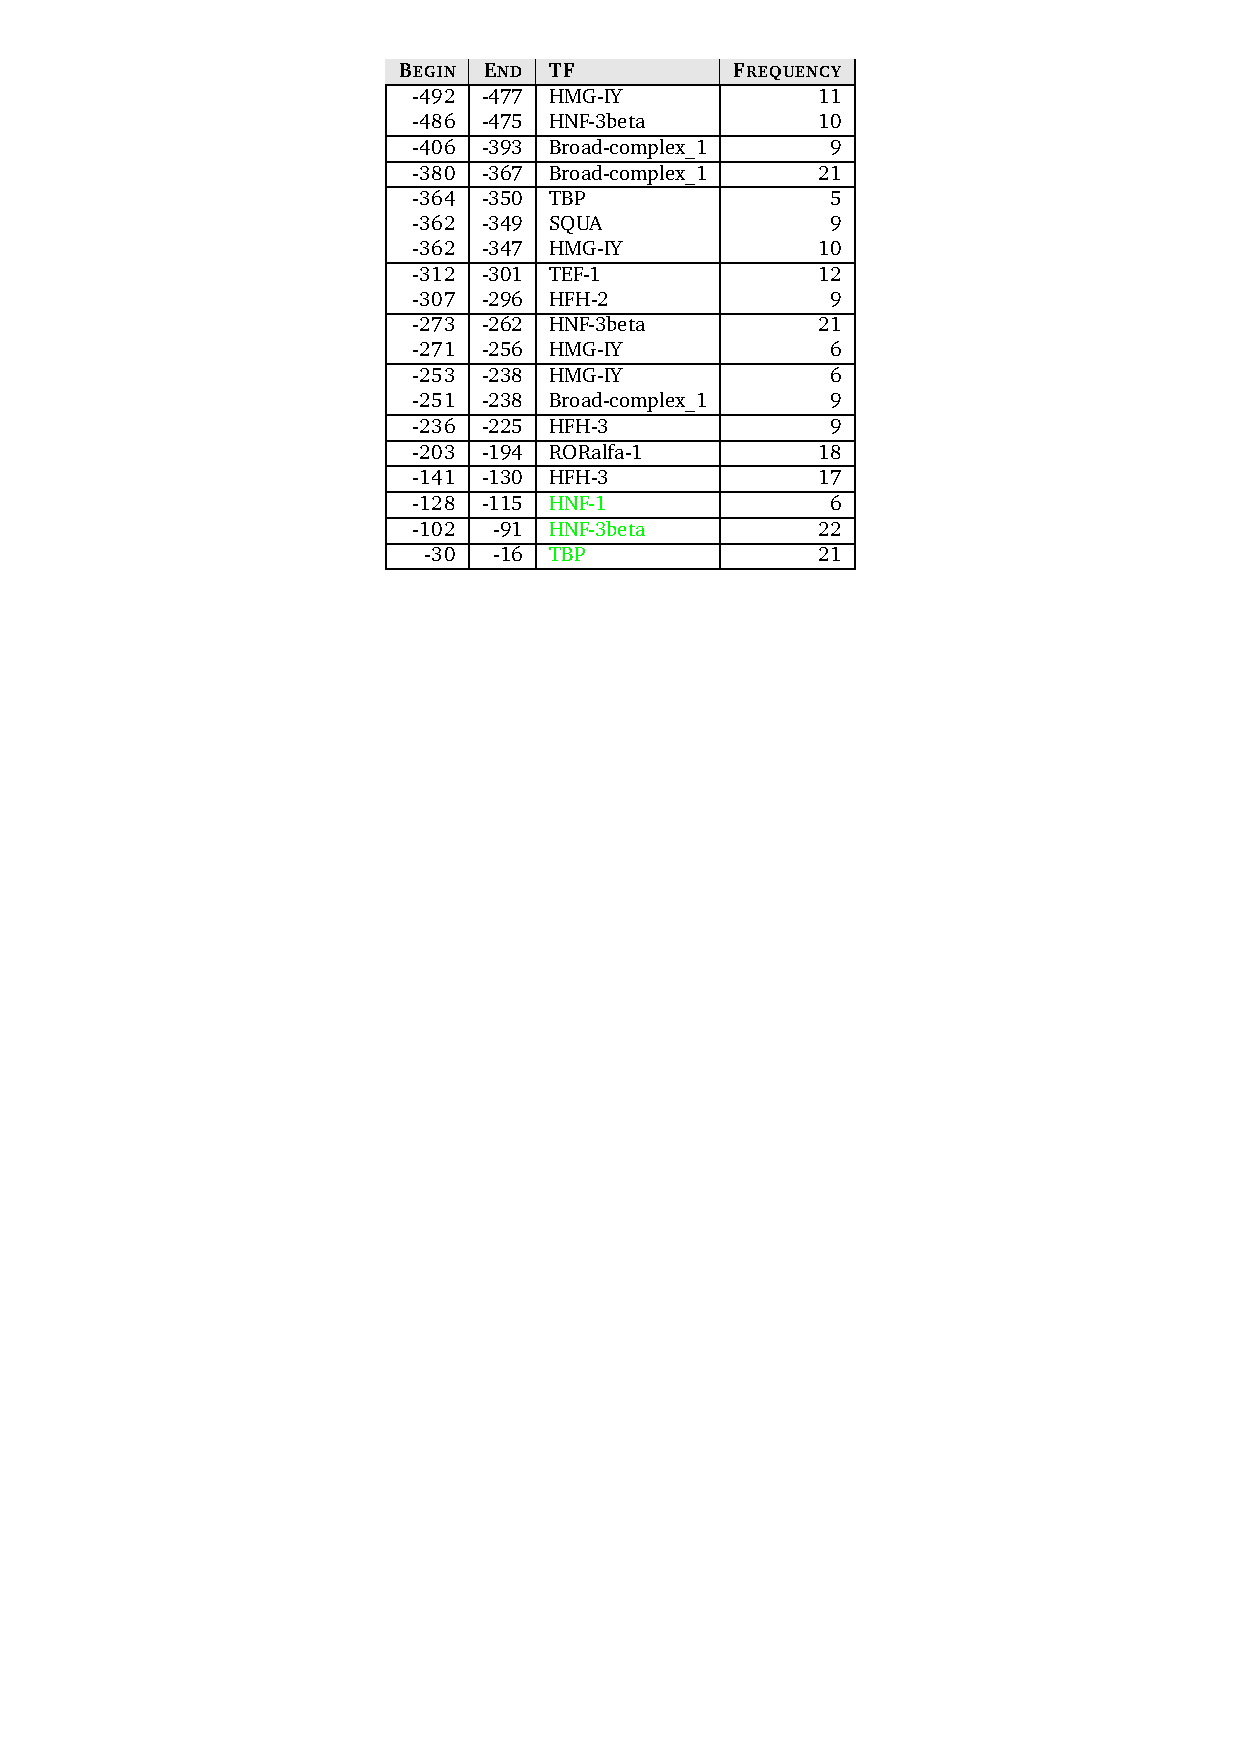
\includegraphics[bb=181 566 414 817,clip]{tables/ttr}
\end{center}
\end{minipage}
\mycaption{tab:ttr}% label
          {Reconstruction of the TTR gene promoter}% lof
          {TF-map alignment reconstruction of the TTR gene promoter.}% caption header
          {Summary of the TF-map alignments obtained between the
promoter of the \emph{transthyretin} gene (TTR, \ensembl{} entry ENSG00000118271)
and the promoters of the genes co-regulated with it according to the CISRED 
database. The table lists the predicted transcription factors on the promoter 
of \emph{transthyretin}, which appear at least in five TF-map alignments with
co-regulated genes. The experimentally verified sites are highlighted.}
\end{center}
\end{table}

It could be argued that the superiority of the TF-map over sequence
alignments has little to do with the alignments and more to do with the
maps. In other words, we would have obtained similar results if we
were to simply score the proportion of TF labels common to the
compared promoter regions --without the need for an
alignment. Therefore, we have computed such a score for each pair of
genes in CISRED: if $p$ and $q$ are the sets of elements in the 
TF-maps of the promoters to be compared, we have computed  
${|p \cap q|^2} / {|p| \cdot |q|}$, where $|p|$ is the size
(cardinality) of the set $p$. Among the 445,371 top scoring
comparisons, 1072 corresponded to co-regulated genes
(with only 394 gene comparisons in common with the TF-map alignment approach), 
a value intermediate between that obtained with sequence and with TF-map
alignments. This reflects that conservation of the relative position of
the TFs along the primary sequence, and not only
common presence, is indicative of gene co-regulation. Conservation of
relative position can only be captured by TF-map alignments.

As an example, Table \ref{tab:ttr} summarizes the TF-map alignments
obtained when aligning the promoter region of the \emph{transthyretin}
gene (TTR, \ensembl{} entry ENSG00000118271) with that of its
co-regulated genes in CISRED. TTR is a serum carrier protein expressed
in liver and brain. The regulatory regions that control the TTR
expression in liver have been experimentally determined \citep{costa:1989a}, 
and consist of a 100-nucleotide enhancer located at -2000 nucleotides 
upstream of the TSS and
a proximal promoter region between -200 and -90 nucleotides upstream of the TSS
(relative to the coordinates in the \ensembl{} entry).
This proximal region is constituted of 6 binding
sites (coordinates relative to TSS of the \emph{transthyretin} 
gene as in the \ensembl{} database): HNF-1 (-137,-109),
HNF-3 (-140,-128 and -106,-91), HNF-4 (-151,-140), C/EBP binding
(-195,-177 and -135,-112). The TATA box is located at -30.
CISRED lists 105 genes co-regulated with TTR. Interestingly, while
BLASTN is unable to detect any sequence 
similarity between the promoter of TTR and that of its co-regulated
genes,  TF-map alignments are obtained in 83
cases, and scored significantly (p-value $<$ 0.001). We have 
reconstructed the structure of the TTR promoter from
the elements that appear in the TF-map alignments. 
A total of 35 TFBSs were initially mapped with \db{Jaspar}$_{TOP50}$ in the 
TTR promoter. For each predicted TF, Table \ref{tab:ttr} lists the number of 
TF-map alignments between TTR, and its co-regulated genes in which the TF appears. 
Only elements appearing in at least five alignments are reported. No matrices 
for the detection of C/EBP and HNF-4 were included in the \db{Jaspar}$_{TOP50}$ collection 
that was used to perform the test. However, the meta-alignments were 
overrepresented in the other experimentally annotated sites, HNF-1, HNF-3 and TATA,
exactly in the region were promoter activity has been reported
(see Figure \ref{fig:ttrannot}). The binding of HNF-3 to positions -140,-128 
is not directly reported. The
TF-map alignments, however, are highly enriched in the HFH-3 factor 
(HNF3/fork head homolog) at this region. In fact, both share a similar 
consensus binding sequence in \db{Transfac} \citep{matys:2003a}: TRTTTRTTT for 
HFH-3 and TRTTTRYTT for HNF-3. 

%%%%
% Figure 14: TTR promoter
%%%%
\begin{figure}[t!]
\begin{center}
\setlength{\fboxsep}{0pt}
\fbox{\incgraph{width=0.75\linewidth}{ps/ttr}}
\mycaption{fig:ttrannot}% label
          {Experimental annotation of the TTR gene}% lof
          {Experimental annotation of the TTR gene promoter.}% caption header
          {Binding sites for activators that control transcription of the mouse 
           \emph{transthyretin} (TTR) promoter in hepatocytes are shown. Adapted from \citep{lodish:2000a}.}
\end{center}
\end{figure}

\subsubsectionblue{Fast computing of all the CISRED TF-map alignments}

For the results of this section, it was necessary to perform 
$5,333 \times 5,333 = 28,440,889$ pairwise TF-map alignments. These combinations 
can be represented into a similarity matrix that is addressed by 
the $5333 \times 5333$ CISRED gene promoter comparison indexes. 
As the similarity between two maps $A$ and $B$ is equal to the
similarity between $B$ and $A$, we only needed to compute $\frac{5333 \times 5333}{2}$
alignments (the other half of the matrix is symmetrical). The alignment
between a gene and itself is also discarded. However, such a number of
alignments is still too high to perform this test several times to evaluate
different conditions in a reasonable amount of time. 

Following the same strategy of the program \prog{pgws} shown in the section before, 
we have divided the work load into different processors. Thus, we have assigned
a part of the similarity matrix to each node taking. Let $G=(g_1,g_2 \ldots g_{5333})$ be
the CISRED collection of gene promoters. A possible planning of tasks based on dividing 
such a matrix by rows into several parts may be: the alignments between the genes 
$g_1 \ldots g_{1000}$ and all of the genes for a first processor; the alignments between the 
genes $g_{1000} \ldots g_{3000}$ and all of the genes for a second processor; the alignments 
between the genes $g_{3000} \ldots g_{5333}$ and all of the genes for a third processor.

The number of assigned rows is different for each processor as the number of alignments that must
be computed for a row is different depending on the part of the matrix is located. For a given 
row $g_i$ in the matrix, only the alignments between such a gene and the genes 
$g_{i+1} \ldots g_{5333}$ must be performed.

After this process, each alignment between two gene promoters $g_i$ and $g_j$ is classified
into $coreg(g_i)$ or $\overline{coreg}(g_i)$ whether the pair $(g_i,g_j)$ is co-regulated
or not according to the CISRED collection.

\clearpage
\sectiongreen[TF-map alignments and matrix specificity]{TF-map alignments and matrix specificity}\label{sec:matrices}

\index{position weight matrices!spe@specificity}

Throughout this chapter, we have used in many experiments smaller subsets of the full collections 
of matrices (e.g. \db{Jaspar}$_{TOP50}$). This fact was explained because of the poor specificity
of many of these matrices in \db{Jaspar} or \db{Transfac}. Several theoretical and practical studies 
have concluded there is a great amount of redundancy in these collections \citep{rahmann:2003a,schones:2005a}. 
In this section, we have numerically explored the specificity of current matrices, using the 
TF-map alignment to obtain similar conclusions.

Position Weight Matrices (PWMs, see Chapter \ref{sec:genefinding} and Figure \ref{fig:pwmsnew}
for a review) have been traditionally used to characterize families of TFBSs. New sequences can 
be analyzed with this model in order to locate putative occurrences of the represented regulatory 
element. However, the ambiguous nature and the short length of the binding sites usually induce
an overwhelming amount of false positive predictions in the searching process.

%%%%
% Figure 15: PWMs construction and use
%%%%
\begin{figure}[t!]
\begin{center}
\setlength{\fboxsep}{0pt}
\fbox{\incgraph{width=0.65\linewidth}{ps/pwmsnew}}
\mycaption{fig:pwmsnew}% label
          {Construction and use of a PWM}% lof
          {Construction and use of a PWM.}% caption header
          {(1) Collect a family of experimentally verified binding sites. 
           (2) Align the sites to find conservations (anchored alignment).
	   (3) Build a weight matrix representation of the alignment: 
           Determine the optimal length; 
	   Define a Threshold value;
           Using a background model, construct the likelihood ratio matrix.
           (4) Search new occurrences of this signal in other sequences.}
\end{center}
\end{figure}

High conservation in certain positions of a PWM may be relevant for the activity of the site. 
Base frequencies may be proportional to the binding energy contribution of the bases. The 
information content of a PWM introduced in Chapter \ref{sec:genefinding} can be used as a 
estimation of its specificity. However, this fact is not always true.

To determine the specificity of current weight matrix models in a genome-wide scale, we have
used protein-coding sequences (CDS) as a negative control. No TFBSs are expected to be
functional in the CDS regions. For the 21,538 genes in the UCSC hg17 human genome release,
we have extracted 500 nucleotides upstream the TSS (PROMOTER samples) and 500 nucleotides 
downstream the Start Codon (CDS samples). 

%%%%
% Figure 16: PWMs QVAL
%%%%
\begin{figure}[t!]
\begin{center}
\setlength{\fboxsep}{0pt}
\begin{tabular}{|cc|}
\hline
\db{JASPAR} & \db{TRANSFAC}\\
\incgraph{width=0.45\linewidth}{ps/qmat1} &
\incgraph{width=0.45\linewidth}{ps/qmat2}\\
\hline
\end{tabular}
\mycaption{fig:qmatrices}% label
          {The $Q-$value distribution in \db{Jaspar} and \db{Transfac}}% lof
          {The $Q-$value distribution in \db{Jaspar} and \db{Transfac}.}% caption header
          {In red, the matrices that produced more predictions in the CDSs; in green,
           the matrices that produced more predictions in the promoters.}
\end{center}
\end{figure}

For each matrix $x$ in \db{Jaspar} 1.0 and \db{Transfac} 6.3, we obtained the number of predicted TFBSs 
in both sets of human samples (Threshold = 0.80): $f_{\textnormal{\scalebox{0.5}{PROM}}}(x)$ and 
$f_{\textnormal{\scalebox{0.5}{CDS}}}(x)$. Next, we define the function $Q$ as the log-likelihood 
ratio between both numbers:

\begin{center}
\fcolorbox{white}{verylightgreen}{
\begin{minipage}[][][c]{0.95\linewidth}
\begin{equation}
Q(x) = log{~~ \frac{f_{\textnormal{\scalebox{0.5}{PROM}}}(x)}{f_{\textnormal{\scalebox{0.5}{CDS}}}(x)}}.
\end{equation}
\end{minipage}}
\end{center}

In Figure \ref{fig:qmatrices}, the distribution of the 
PWMs in \db{Jaspar} and \db{Transfac} according to this measure is shown. Not surprisingly, 40\% of the 
\db{Transfac} matrices (37\% in \db{Jaspar}) produced even more predictions in the CDS sequences than 
in the actual promoter regions (see Table \ref{tab:qmatrices}). For different values of
$Q$, more strict sets of matrices can be obtained, as shown in Table \ref{tab:qmatrices}.

The test we performed on the \textsc{HR set} (see Figure \ref{fig:testregions}) showed that 
TF-map alignment could distinguish two orthologous promoters better than any other
pair of orthologous genomic samples, even with lower sequence similarity (see Section 
\ref{sec:testregions} for further details). \db{Jaspar}$_{TOP50}$ was used as a mapping function,
because the $50$ most informative matrices in \db{Jaspar} were supposed to be the more specific.
In fact, we can now quantify the optimal number of matrices (and which matrices) to achieve
the maximum discrimination power, using the $Q$-value function.

As we are going to align human-mouse pairs, we have also computed the $Q$-value using the mouse 
genome (17,213 genes, mm5) for the complete collection of matrices in \db{Jaspar} and \db{Transfac}, 
following the procedure explained above for the human genes. For each $Q$-value, we have
intersected the subset of matrices according to the human and the mouse genomes. Then, we have 
repeated the test detailed in Section \ref{sec:testregions} using these different sets of matrices.
The test with the full collections was also performed to compare against the smaller subsets.

Table \ref{tab:qmatrices2} lists the number of times each genomic region (promoter, 5'UTR, CDS,
intronic, intergenic, downstream) scores the highest in each gene of the \textsc{HR set} using
each subcollection of matrices. It is remarkable that the $Q \geq 0.5$ in \db{Jaspar}, with only 
$16$ matrices, identified correctly $20$ of the promoter pairs. Notice the poor performance
when we used the full \db{Jaspar} collection. In fact, the results do not improve when we add or 
remove other matrices to the optimal subset of matrices. Similar results are obtained when
we used \db{Transfac}. The optimal collections are listed in Table \ref{tab:qcollections}. In
both cases, the majority of the matrices are the most informative. Despite this, some 
significant matrices with a small information content are also included in both optimal sets
(e.g. the SP1 matrix in \db{Jaspar} and \db{Transfac}). As in the previous test, we performed
the global alignment to show the sequence similarity of each sample pair
with the program \prog{needle} of the EMBOSS software \citep{olson:2002a}.

Finally, it is important to mention that the subset of matrices that we arbitrarily
selected in the original test (\db{Jaspar}$_{TOP50}$, see Section \ref{sec:testregions}) 
obtained slightly better results than the optimal set estimated with the $Q$-value method.
This subset, however, only have 16 matrices, while \db{Jaspar}$_{TOP50}$ is constituted of
$50$ matrices.

%%%%%%%%%%%%%%%
%%% TABLE 6
%%%%%%%%%%%%%%%
\begin{table}[t!]
\begin{center}
\begin{minipage}{0.98\linewidth}\setlength{\parindent}{0pt}
\begin{center}
\scalebox{0.85}{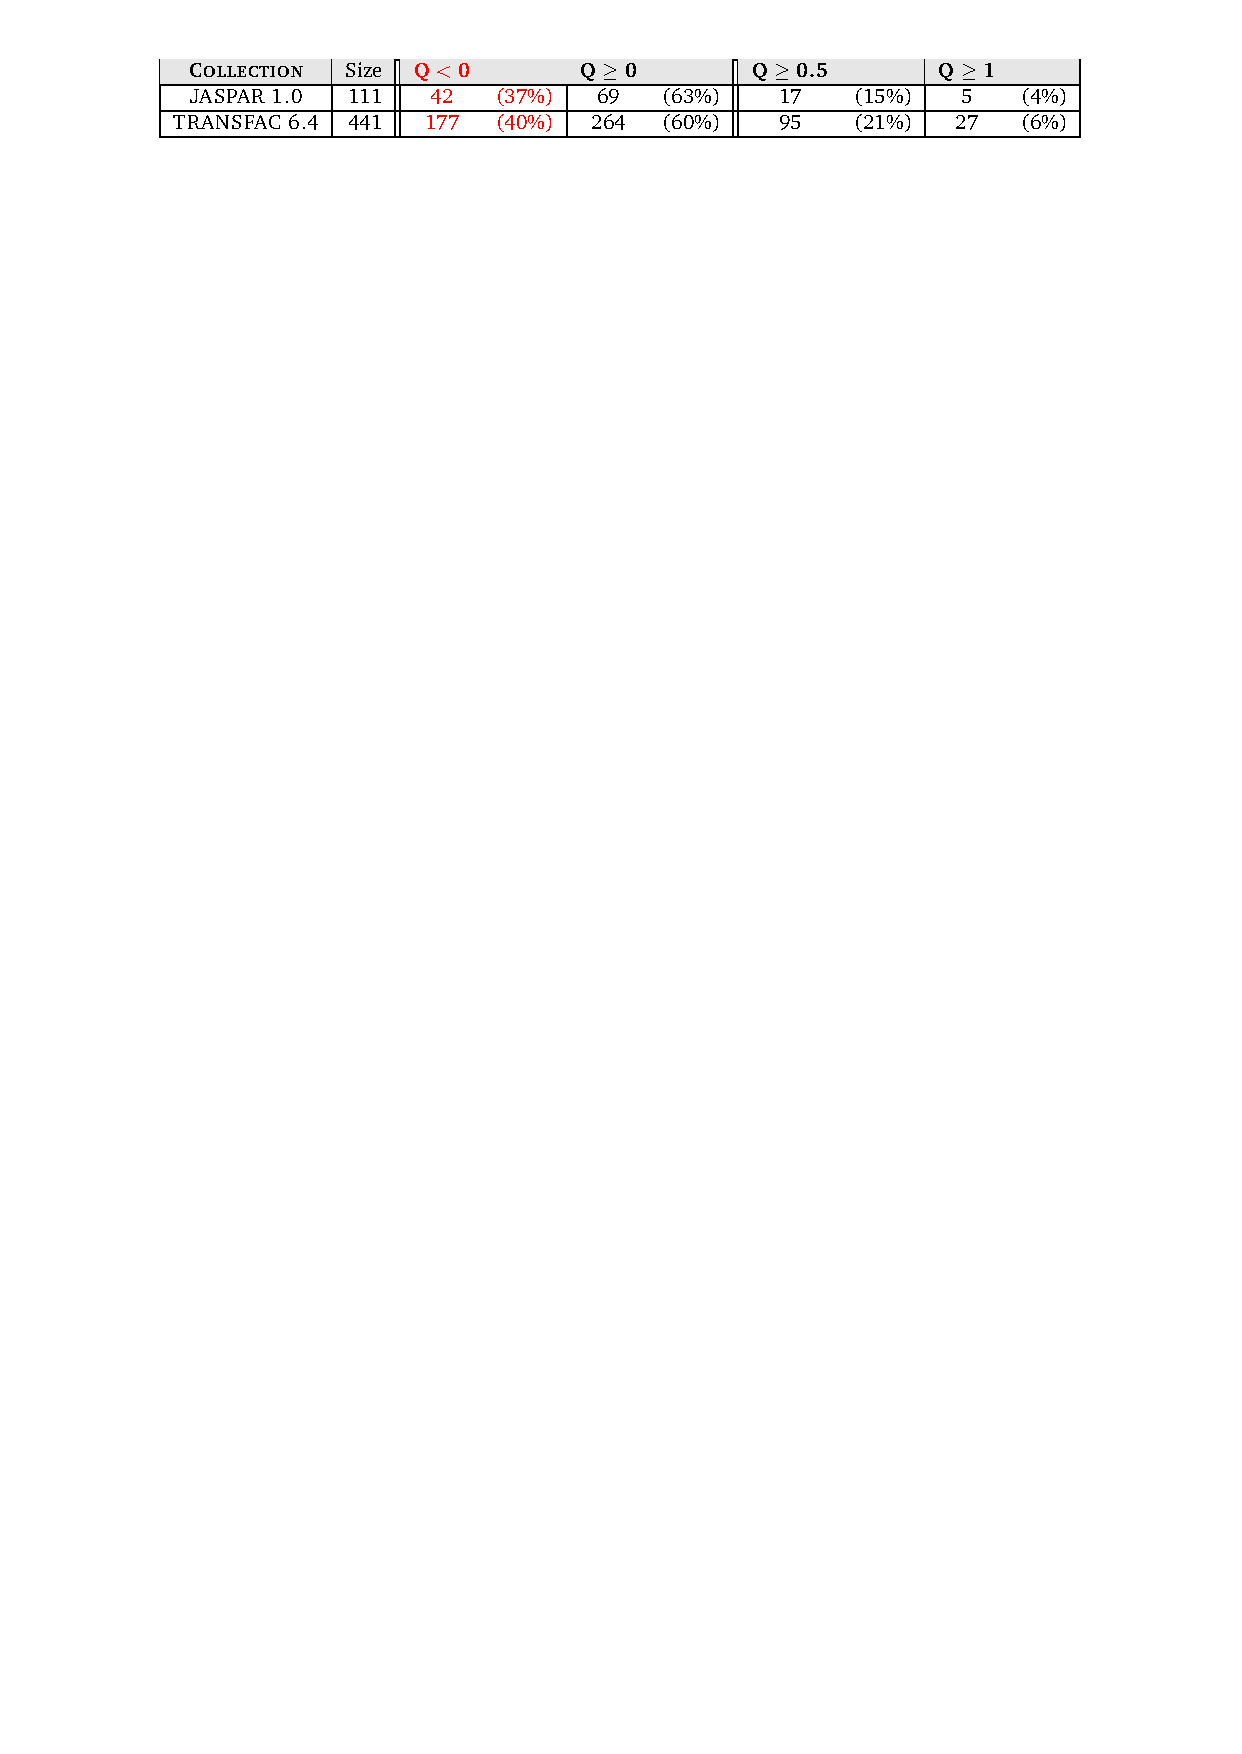
\includegraphics[bb=74 775 522 816,clip]{tables/qvalue}}
\end{center}
\end{minipage}
\mycaption{tab:qmatrices}% label
          {$Q$-value and PWM matrix specificity}% lof
          {$Q$-value and PWM matrix specificity in \db{Jaspar} and \db{Transfac}.}% caption header
          {}
\end{center}
\end{table}

Several conclusions can be extracted, therefore, from this simple test:
\begin{enumerate}
\item
Up to 40\% of the matrices from popular matrices repositories are prone to predict the same 
number of TFBSs either in human promoters or in protein coding sequences. Therefore, analysis 
with these models must be very carefully evaluated.
\item
Although a high information content normally implies better specificity of the matrices, 
there are cases in which both characteristics are not related.
\item
The use of complete collections to analyze homologous promoters usually produces the
recognition of artefactual sequence conservations as shown when the matrices are
applied on protein coding regions or intron sequences.
\item
To locate the actual common regulatory elements in a set of co-expressed sequences, it is
advisable to restrict the search using smaller collections of matrices. A simple procedure
to detect those matrices that consistently appear more frequently in a set of co-regulated
genes than in a negative control set can provide interesting results.
\item
Many of the numerous drawbacks of the weight matrices such as redundancy and low specificity
are caused by the simplicity of the model. Therefore, the use of more complex models to incorporate
additional information will obviously improve future predictions. However, we also suggest a more
rational application of the current systems to enhance the advantages and to mask the inconveniences
of these representations.
\end{enumerate}


%%%%%%%%%%%%%%%
%%% TABLE 7
%%%%%%%%%%%%%%%
\begin{table}[t!]
\begin{center}
\begin{minipage}{0.98\linewidth}\setlength{\parindent}{0pt}
\begin{center}
\scalebox{0.75}{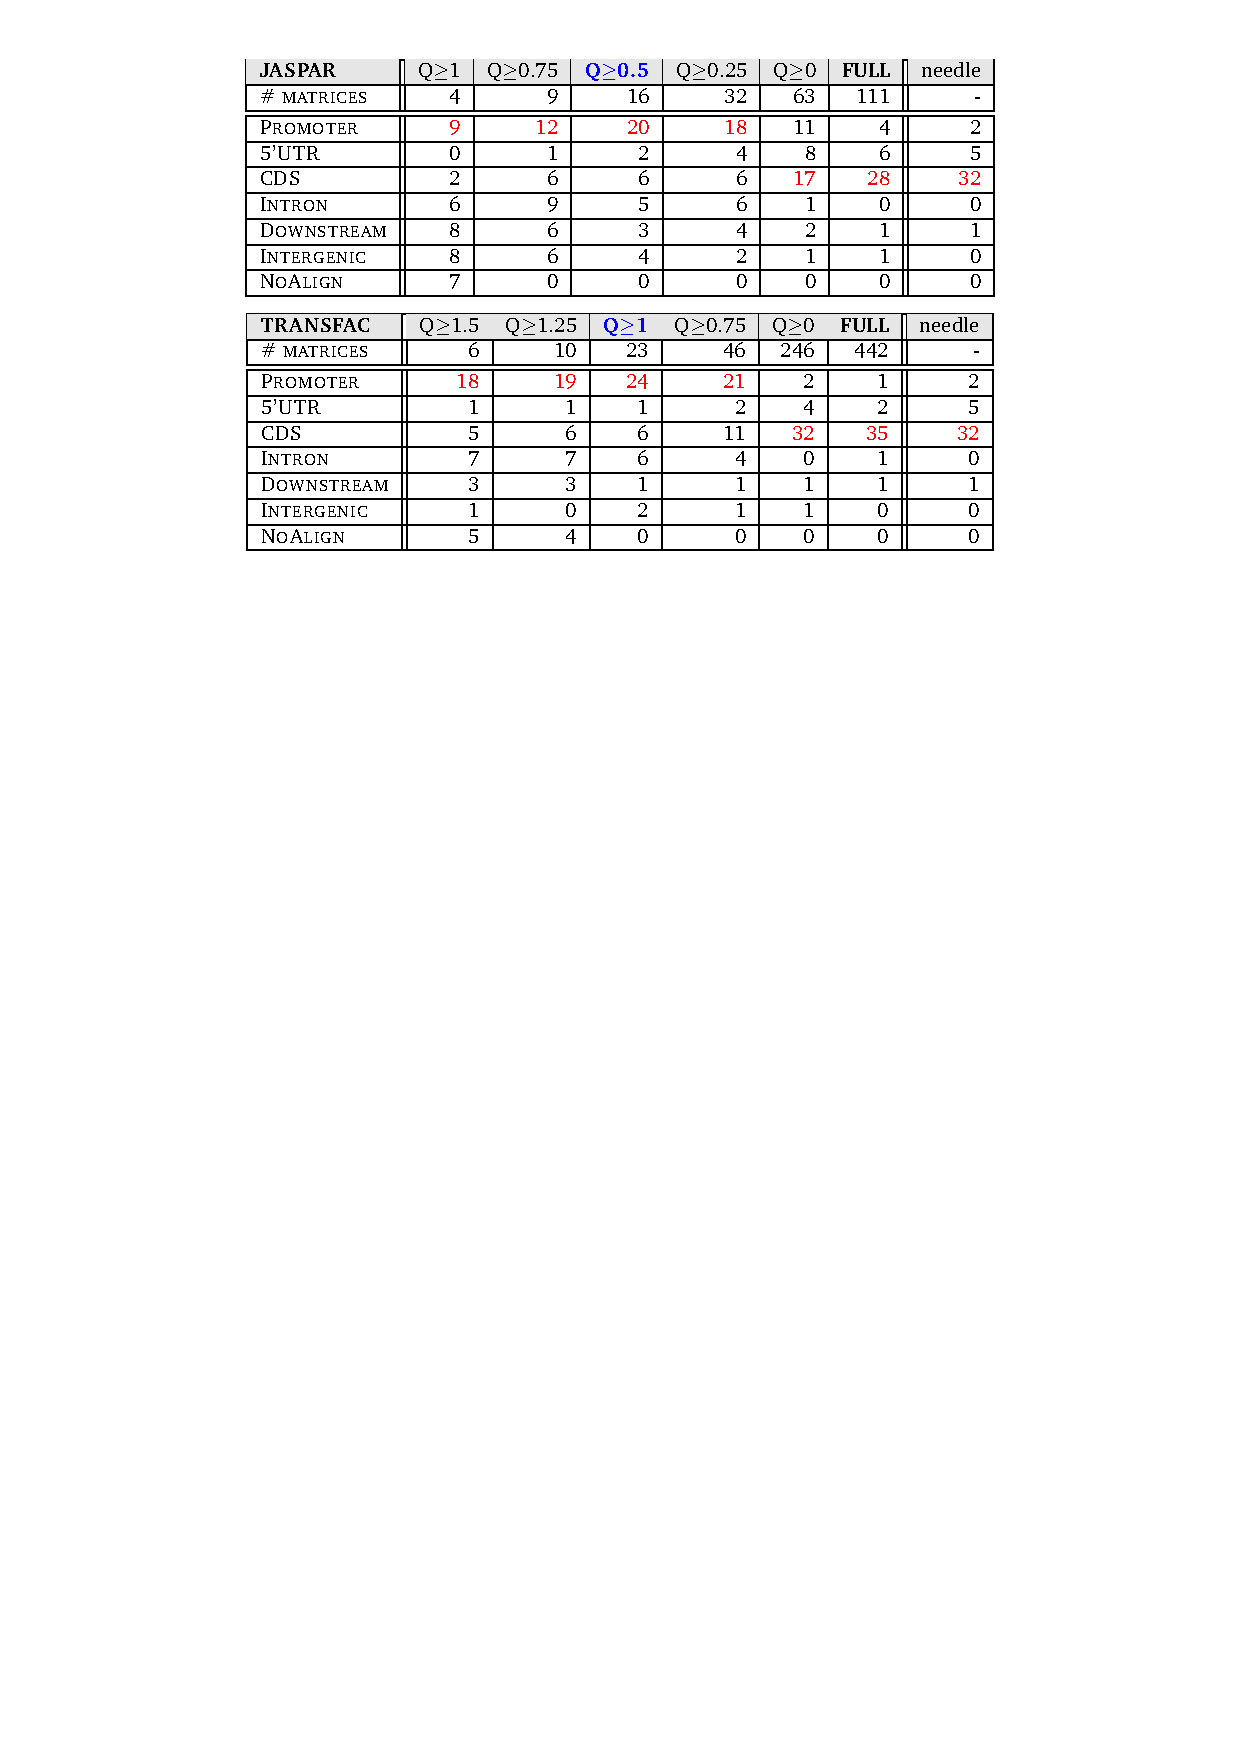
\includegraphics[bb=115 574 480 817,clip]{tables/qvalue2}}
\end{center}
\end{minipage}
\mycaption{tab:qmatrices2}% label
          {Evolution of the matrix specificity}% lof
          {Matrix specificity in several subsets of \db{Jaspar} and \db{Transfac}.}% caption header
          {}
\end{center}
\end{table}

%\sectiongreen{Meta-alignment in other scenarios}
%- IMPORTANTE: Este es un algoritmo generico que procesa cualquier tipo de informacion
%- hacer pruebas sobre ejemplos de datos en otros ambitos: AFIS, comparar otro tipo de mapas,
%comparacion de imagenes para extraer patrones????

\sectiongreen{Local TF-map alignments}

\index{TF-map alignments!loctf@local}
Local alignments are very useful to identify short stretches of a sequence that
are conserved in another one, despite the rest of both sequences is probably different. 
Local comparisons are also interesting mechanisms to locate the location (if any) of
a short composite (cluster of TFBSs, a super-pattern of TFBSs) in a long TF-map 
(see Figure \ref{fig:ttrc}). 

Two alternative designs were presented in Chapter \ref{sec:algorithms} (Section \ref{sec:local})
to implement a sequence local alignment according to the scoring function: similarity or
distance. Based on them, we present here two different implementations to identify local 
meta-alignments between two TF-maps.

\subsectionblue{Local TF-map alignments using similarity}

In a short communication, \citet{smith:1981c} published a slight modification of the 
\citeauthor{needleman:1970a} algorithm, as revisited by \citet{smith:1981b}, to deal with 
local alignments. The main objective is to find the pair of segments, one from each of two 
long sequences, such that there is no other pair of segments with greater similarity (homology).

The basic rationale of this strategy is the following: let $S(i,j)$ a position in the dynamic
programming matrix. The best local alignment ending at $S(i,j)$ is computed according to the 
three adjacent values in the matrix $S$ as long as the incorporation of one of these elements 
does not produce an alignment with negative homology. In that case, the score of the alignment 
ending at $S(i,j)$ is set to $0$. The traceback procedure then starts from the matrix cell 
having the maximum similarity, constructing the best local alignment until a cell that contains
a $0$ is reached.

%%%%%%%%%%%%%%%
%%% TABLE 8
%%%%%%%%%%%%%%%
\begin{table}[t!]
\begin{center}
\begin{minipage}{0.98\linewidth}\setlength{\parindent}{0pt}
\begin{center}
\scalebox{0.8}{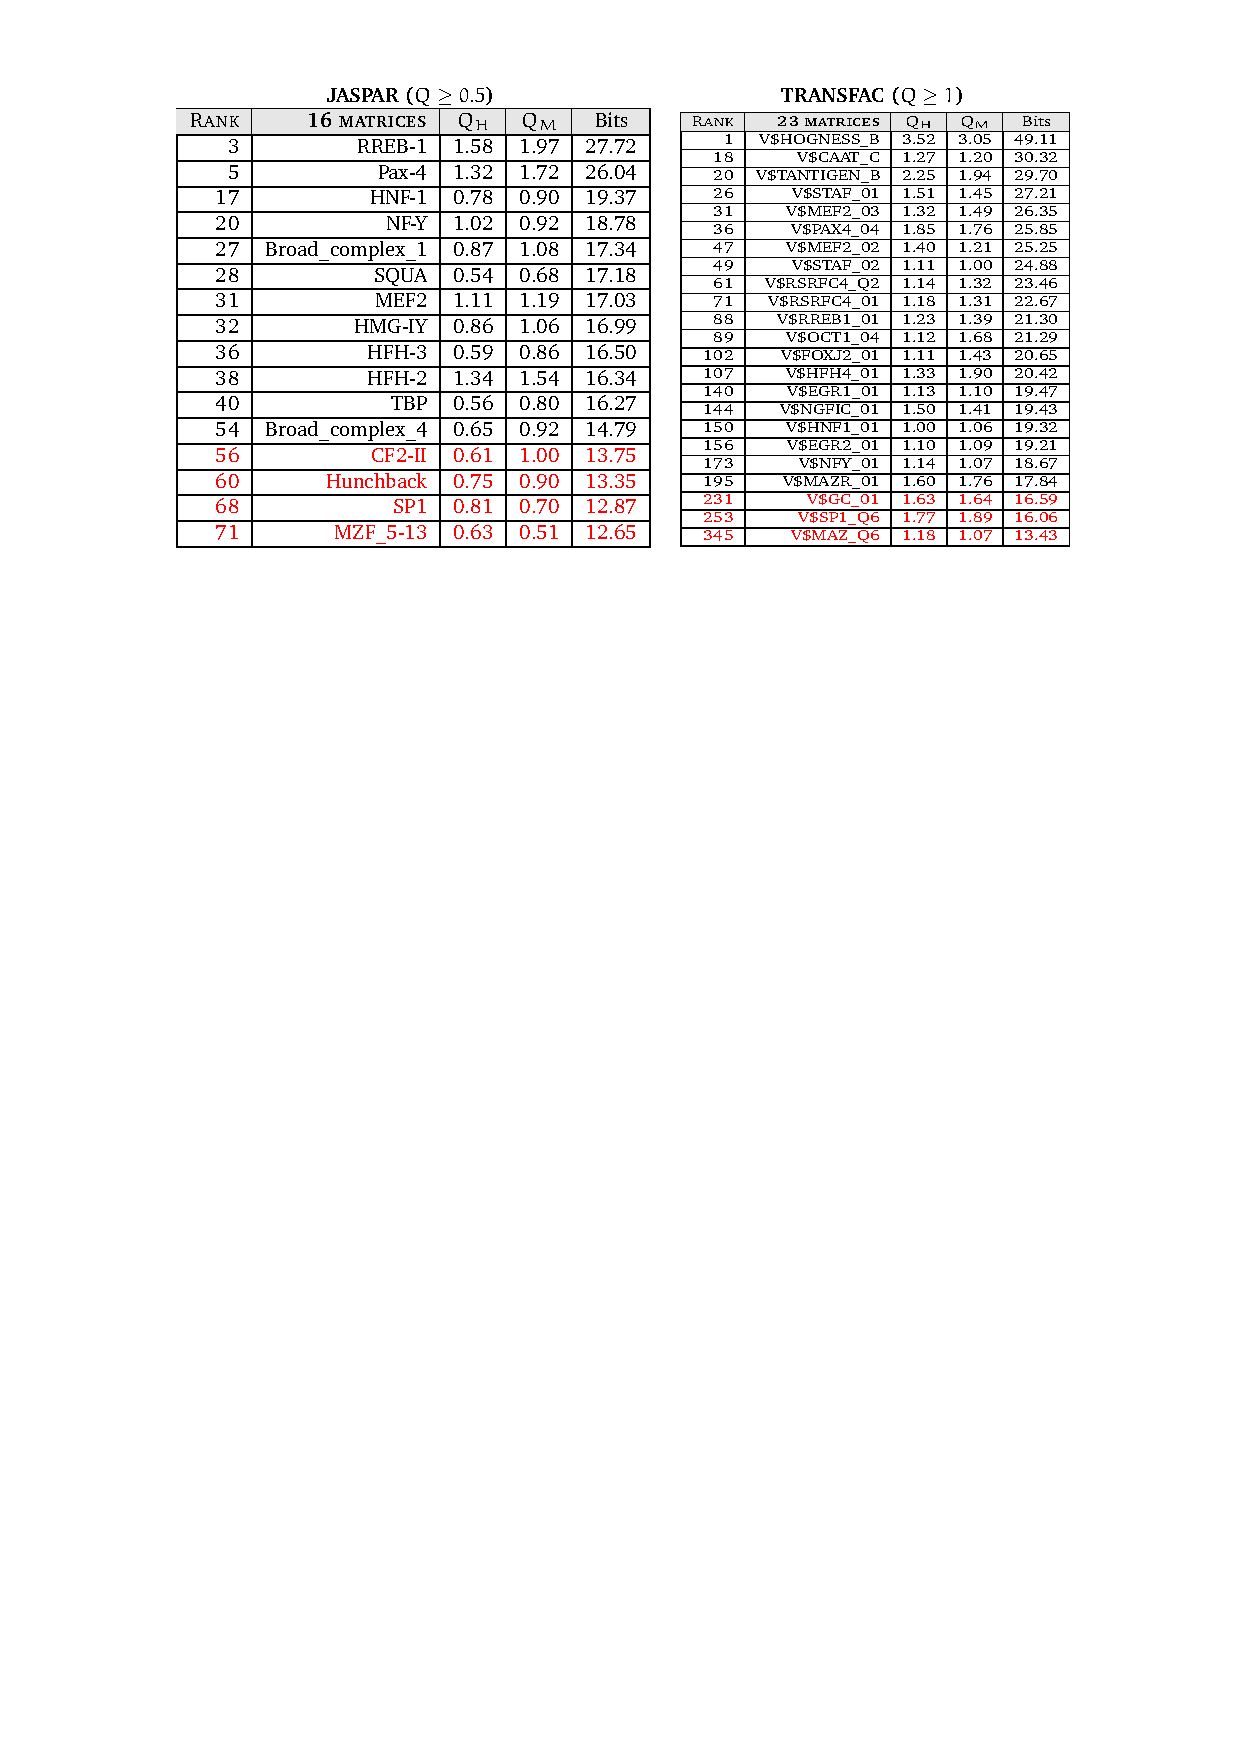
\includegraphics[bb=82 578 518 817,clip]{tables/qcolls}}
\end{center}
\end{minipage}
\mycaption{tab:qcollections}% label
          {\db{Jaspar} and \db{Transfac} specific subsets}% lof
          {\db{Jaspar} and \db{Transfac} specific subsets.}% caption header
          {In red, the matrices that are not among the most informative ones.}
\end{center}
\end{table}

The application of this approach to the meta-alignment is trivial. We can rewrite the
Equation \ref{eqnaive} introducing the $0$ in the appropriate place to produce the local alignment.
Thus, the maximum local similarity $S_{ij}$ between TF-maps  $A = a_1 \ldots a_i$ and 
$B = b_1 \ldots b_j$ where the site $a_i^f$ is equal to the site $b_j^f$, 
can be computed as: 

\begin{center}
\fcolorbox{white}{verylightgreen}{
\begin{minipage}[][][c]{0.95\linewidth}
\begin{equation}
\begin{array}{lllll}
S_{ij} \equiv & S(a_i,b_j) = & max \{0,& \alpha (a_i^s + b_j^s) +& \\
              & & &  max_{i',j'} & \{S_{i'j'}\\
              & & & \scalebox{0.7}{\mbox{$0 < i' < i$}} & - \lambda (i - i' - 1 + j - j'- 1)\\
              & & & \scalebox{0.7}{\mbox{$0 < j' < j$}} & - \mu (|(a_i^{p_1} - a_{i'}^{p_1}) - (b_j^{p_1} - b_{j'}^{p_1})|)\}\}.\\
              & & & \scalebox{0.7}{\mbox{$a_{i'}^{p_2} < a_i^{p_1}$}} & \\
              & & & \scalebox{0.7}{\mbox{$b_{j'}^{p_2} < b_j^{p_1}$}} &  
\end{array}
\end{equation}
\label{eqlocal}
\end{minipage}}
\end{center}

If we save the $N$ positions in $S$ that have the best score, we can report the best $N$ local
alignments or blocks between $A$ and $B$. The cost of the algorithm is the same as in the
global TF-map alignment algorithm, as no additional operations are necessary.

\subsectionblue{Local TF-map alignments using distance}

Despite the solution to the problem of local meta-alignment using similarity is simple
and clear, we also decided to investigate the form to produce local alignments under
the original distance scheme framework \citep{waterman:1984c}. We have taken advantage of
this research to study in depth the distribution of the scores (distance) in the meta-alignments.

As reviewed in Chapter \ref{sec:algorithms} (Section \ref{localdist}) the solution
developed by \citet{smith:1981c} to produce local alignments using a similarity
scoring function can not be directly applied in the case of the distance metric.
\citet{goad:1982a} defined the mismatch density of the alignment between two segments as 
the ratio of the minimum distance $D$ between both sequences and the length $L$ of such 
an alignment. Thus, only those alignments with a mismatch density below a certain positive 
threshold $T$ should be reported.

Formally, we are interested in those paths in the dynamic programming distance matrix
such that the mismatch density on them is minimal. The length of these alignments is a 
priori unknown and can be variable. The value of the threshold $T$ is different for each 
input, having a statistical and biological meaning at the same time.


%%%%
% Figure 17: GFF2PS: localizar un patron en una entrada
%%%%
\begin{figure}[t!]
\begin{center}
\setlength{\fboxsep}{0pt}
\fbox{\incgraph{width=0.7\linewidth}{ps/ttrc}}
\mycaption{fig:ttrc}% label
          {Using local meta-alignment in pattern identification}% lof
          {Using local meta-alignment to identify known patterns in orthologous sequences.}%header
	  {(Top) TF-map obtained with \db{Jaspar}$_{TOP50}$ on the chicken promoter of the TTR gene, 
           and a second map of three experimentally verified TFBSs in the human ortholog. 
           (Bottom) The local alignment between both maps identifies the putative 
           location of the human sites in chicken.}
\end{center}
\end{figure}

This is the procedure we follow to obtain the local meta-alignment between two maps $A$ and $B$
(see Figure \ref{fig:locprot}):

\begin{menumerate}
\item
Compute the global alignment of both maps (distance metrics), to fill the 
dynamic programming matrix $D$ in. Each position $D(i,j)$ contains the 
minimum distance in terms of a meta-alignment between the map $A = a_1 \ldots a_i$ 
and the map $B = b_1 \ldots b_j$. 
\item
Compute the matrix $\Delta D$ from $D$. For each two consecutive nodes in the
matrix $D(i,j)$ and $D(i',j')$ that are part of a path, we compute the increase 
of the distance value produced by adding the second match after the first one:

\begin{center}
\fcolorbox{white}{verylightgreen}{
\begin{minipage}[][][c]{0.95\linewidth}
\begin{equation}
\Delta D(i,j) = D(i,j) - D(i',j') ~\mbox{where}~ i' < i, j' < j.
\end{equation}
\end{minipage}}
\end{center}

\item
Define the threshold $T$ according to the $\Delta D$ values in the alignments
of length $L=2$ TFBSs. We define this threshold taking into account that
the distribution of the distance in such alignments follows the Gumbel
or extreme-value distribution (see Figure \ref{fig:glocal}). The Gumbel
function is defined as:

\begin{center}
\fcolorbox{white}{verylightgreen}{
\begin{minipage}[][][c]{0.95\linewidth}
\begin{equation}
y = e^{-x-e^{-x}} ~\mbox{where}~ P(x<0) = 0.368, P(x>0) = 0.632.
\end{equation}
\end{minipage}}
\end{center}

We are interested in defining $T$ such that a small fraction of the smallest 
values is selected. The normalization of a Gumbel function is computed as:

\begin{center}
\fcolorbox{white}{verylightgreen}{
\begin{minipage}[][][c]{0.95\linewidth}
\begin{equation}
z = \lambda (x - \mu) ~\mbox{where}~ \lambda = \frac{1.285}{\sigma}, \mu = \overline{x} - 0.45 \sigma.
\end{equation}
\end{minipage}}
\end{center}

$\overline{x}$ and $\sigma$ are the mean and the deviation of the distance values computed for 
the current set of paths, respectively. If we are considering the values $P(z \leq Z) = 0.05$,
that is under 5\% of the area covered by $z$, then:

\begin{center}
\fcolorbox{white}{verylightgreen}{
\begin{minipage}[][][c]{0.95\linewidth}
\begin{equation}
\begin{array}{c}
z = \frac{1.285 \cdot x - 1.285\cdot \overline{x} -1.285 \cdot 0.45 \sigma}{\sigma}\\
G(P) = -ln (ln (\frac{1}{p}) ~\mbox{where}~ p = 0.05, \mbox{(value of $z$)}.
\end{array}
\end{equation}
\end{minipage}}
\end{center}

For each alignment input, we will have a different $\overline{x}$ and $\sigma$ values
that, according to this equation, will provide a threshold $T$ to obtain only the
5\% of the minimal distance alignments of length $2$.

\item
Finally, trace back the paths ending at each match in the $\Delta D$ matrix. The
rule to extend a local alignment takes into account a weighted version of the
mismatch density value. A new match is added to the path if the accumulated distance
is below $T$:

\begin{center}
\fcolorbox{white}{verylightgreen}{
\begin{minipage}[][][c]{0.95\linewidth}
\begin{equation}
\frac{\Delta D(i,j)}{l} < T
\end{equation}
\end{minipage}}
\end{center}

where $l$ is the length of the current local alignment path. Visited nodes are marked up 
to be skipped in future path extensions (avoid overlapping of the solutions).
\end{menumerate}

%%%%
% Figure 18: Protocol for local alignment (D)
%%%%
\begin{figure}[t!]
\begin{center}
\setlength{\fboxsep}{0pt}
\begin{tabular}{ccc}
1 & 2 & 3\\
\fbox{\incgraph{height=4cm,width=0.3\linewidth}{ps/posterloc1}} &
\fbox{\incgraph{height=4cm,width=0.3\linewidth}{ps/posterloc2}} &
\fbox{\incgraph{height=4cm,width=0.3\linewidth}{ps/posterloc3}}\\
\end{tabular}
\mycaption{fig:locprot}% label
          {Local meta-alignment using the distance metric}% lof
          {Local meta-alignment using the distance metric}% header
          {(1) Global alignment of both maps. 
           (2) Compute the $\Delta D$ matrix for $L=2$.
           (3) Extend the best local paths with the score below $T$.}
\end{center}
\end{figure}

\sectiongreen{Discussion}

Much of the biology of the past decades has been based on the
technological advances that have accelerated our ability to sequence
DNA and proteins. It is certainly in the sequence of the genome where
the biological traits of organisms are encoded. While we have a
relatively good understanding of some of the basic mechanisms involved
in the processing of the information encoded in the DNA sequence, it
is in general very difficult to predict the biological traits --even at
the molecular level-- from the nucleotide sequence alone. Gene
promoters are a case in point: while the sequence of the promoter is
likely to contain most of the information to control the expression of
a gene, it is currently impossible to predict the expression pattern
of a gene from the analysis of its promoter sequence alone.

%%%%
% Figure 19: Gumbel distribution
%%%%
\begin{figure}[t!]
\begin{center}
\setlength{\fboxsep}{0pt}
\begin{tabular}{cc}
\incgraph{height=8cm,width=0.45\linewidth}{ps/gumbelloc1} &
\incgraph{height=8cm,width=0.45\linewidth}{ps/gumbelloc2}\\
\end{tabular}
\mycaption{fig:glocal}% label
          {Gumbel distribution of local meta-alignments}% lof
          {Gumbel distribution of local meta-alignments.}% header
          {(Left) The Gumbel generic function. (Right) TF-map alignment scores in a real pair of promoters.}
\end{center}
\end{figure}

While inferring function directly from sequence is thus far from
trivial, it is still true, that because sequence encodes function, 
similar sequences often encode similar functions. Sequence comparisons,
therefore, are an extraordinary tool to infer functional relationships: 
through sequence comparisons the function of known sequences can be 
extrapolated to newly obtained ones, and the specific sequence motifs 
can be identified responsible for the common functionality of a set of
sequences. But sequence comparisons have limitations: often
similar functions are encoded by diverse sequences. Again,
gene promoters are a case in point: many TFs bind to
sequence motifs which do not show sequence conservation. Thus, while
through phylogenetic footprinting, conserved regulatory motifs have
been in occasions uncovered in the promoters of orthologous genes
\citep{blanchette:2002a,lenhard:2003a}, searching for common patterns through the comparison of
promoter sequences in sets of co-regulated genes --as, for instance,
those resulting from microarray experiments-- is usually a frustrating
exercise. 

Here, we have attempted to address this limitation implicit in sequence
comparisons, by annotating the primary sequence with predicted
functional domains, comparing the resulting annotations instead of the
underlying primary sequence. If functional domains are encoded by
diverse sequences, the comparison and alignment of the annotation may
be more revealing of the functional relationships between sequences
and of the specific domains involved in the common functionality than
the comparison and alignment of the primary sequence. In particular,
we have attempted this strategy for the comparison and
characterization of promoter regions from genes with similar
expression patterns. We have annotated the sequence with predictions
of TFBSs --using a variety of popular tools and databases-- and identified 
the predicted sites with the labels of the corresponding TFs. We have then
compared and aligned the resulting sequence of labels. Because TFs can
bind to sites that show no sequence conservation, their labels can be
aligned which correspond to domains that, while exhibiting similar
functions, may not show sequence conservation. 

Precedents of this approach can be found in the literature.
\citep{quandt:1996a}, for instance, distinguish explicitly between
first-level analysis of promoters, in which the nucleotide sequence
is directly interrogated for the presence of regulatory motifs, and
second-level methods, in which basic higher order patterns can be
defined from a number of correlated first-level units. This
approach is further developed in \citep{frech:1997a} and
\citep{klingenhoff:1999a}, where more complex composite patterns are derived
capturing the functional organization of individual regulatory elements,
and are then used to identify and characterize related promoter
regions in absence of sequence conservation. 
Here, we go one step further, and infer automatically the composite patterns by
explicitly aligning the sequences of labels corresponding to TFs for
which binding sites have been predicted in the compared promoters (the
second-level annotation).

To align these sequences of labels--to which we refer as TF-maps--
we have stated the problem as a restriction enzyme map alignment, and
adapted a dynamic programming algorithm developed by \citet{waterman:1984c}. 
This algorithm, as well as ours, belong to a larger class of map
alignments algorithms (see also, \citep{miller:1990a,miller:1991a,myers:1992a,huang:1992a}). 
In typical alignments, the sequences are of labels
denoting either nucleotides or amino acids. In map alignments, the
sequences are of pairs (label,integer), where the label denotes a
predicted domain or site (possibly exhibiting some behavior or functionality), 
and the integer the position on the primary sequence where the domain or the 
site has been predicted. In global pairwise sequence alignments, the goal is to
obtain the alignment that maximizes the sum of the scores of the
aligned positions --given the score of the individual alignments of
all possible pairs of labels. In contrast, in map alignments, only
positions with identical labels can be aligned and the goal is to
obtain the largest common subsequence constrained to minimize the
differences in distances on the primary sequence between consecutive
aligned positions. Sequence and map alignments can be generalized to a
broader class of alignments that includes both. 

Map alignments have been mostly used to align restriction enzyme
maps. In this case, the label denotes a restriction enzyme, and the
integer the position on the primary sequence of the site recognized by
the enzyme. \citet{waterman:1984c} first established the concept of
map alignment and provided an algorithm for computing the optimal
alignment of two maps. Later \citet{myers:1992a} described an improved
algorithm to efficiently find map alignments which relies on the
extreme sparsity of the dynamic programming matrix in \citep{waterman:1984c}
--the result of the match state being defined only between identical labels. 
\citet{miller:1990a,miller:1991a} introduced new algorithms that permitted
the efficient search of a long map for the best matches to a shorter probe map.
\citet{huang:1992a} generalized these algorithms to deal with different map errors. 

In our case, the label denotes a TF, and the integer the initial
position on the primary sequence where a binding motif for the TF has
been predicted. There are, however, two important differences between
restriction enzyme maps and TF-maps. First, while prediction of
restriction sites is deterministic, producing a binary output
(``site'', ``no site''), prediction of TFBSs is often probabilistic
and predicted sites may have an associated score. The score can
usually be related to the strength of the binding of the TF to the
site \citep{stormo:2000a}. Since, it makes sense, therefore, to prefer
in TF-map alignments higher scoring sites, the score of the TFBSs needs
to be taking into account when building optimal TF-map alignments.
Second, enzyme restriction sites are single-nucleotide positions on
the primary sequence. TFBSs, in contrast, are sequence intervals, and
have thus, in addition to position, an associated length. Because we
explicitly prohibit overlap between aligned elements, we can not
directly extrapolate the algorithm of \citet{myers:1992a}. However, as
in their approach, we have also taken advantage of the extreme
sparsity of the dynamic programming matrix to implement an efficient
algorithm that, in our experience, is comparable in efficiency. There
is another important feature characteristic of our approach that,
while it does not influence the algorithmic strategy, it is essential
to its success. As we have already stressed, we do not label the site,
but the function of the site. That is, we do not label the TFBSs, but
the TFs that bind to the sites. This allows for significant functional
alignments even in the absence of sequence conservation.

We have estimated the optimal parameters of the algorithm in a small,
but well annotated, set of orthologous human-mouse genes. We used three
popular collections of PWMs for TFBSs (\db{Jaspar} 1.0 \citep{sandelin:2004a}, 
\db{Promo} 2.0 \citep{farre:2003a} and \db{Transfac} 6.3 \citep{matys:2003a}) to 
obtain the TF-maps of the promoter sequences. Results on this data set 
indicate that, by dramatically reducing the overwhelming number of 
spurious predictions of TFBSs produced using these collections, 
TF-map alignments are able to successfully uncover the few conserved 
functionally active regulatory domains. 
Differences can be observed between the performance of the
different collections of TFBSs; alignments obtained using \db{Jaspar}  
--and, in particular, using a subset consisting of the 50 top most informative
matrices-- appear to show the optimal balance between sensitivity and
specificity. The data set that we have used, however, is too small to
infer general trends on the comparative behavior of these collections.

Interestingly, despite the stronger sequence conservation between
protein-coding regions, TF-map alignments score the highest between promoter
regions in the training set of orthologous human-mouse genes. 
This indicates that TF-map alignments are able to pick up regulatory
signals that sequence alignments can not. Results in an independent
larger data set of co-regulated genes from the CISRED database are
also in support of this conclusion: we have been able to obtain more
significant alignments between the TF-maps than between the nucleotide
sequences of the promoters of co-regulated genes. Results in CISRED are
certainly not extraordinary. Both sequence and TF-map alignments
perform very poorly when detecting relationships between co-regulated
gens in CISRED. Only in 97 out of 5333 gene representatives in CISRED
(1.8\%), TF-map alignments scored significantly higher for co-regulated 
than for non co-regulated genes. Using BLASTN, this number was only 11
(0.2\%). Finding relationships between the promoters of the genes
co-regulated in CISRED is a task as challenging as one can
imagine. The CISRED collection of high-confidence co-expressed genes
is not derived from overall conservation, or from co-occurrence of motifs, 
in the sequence of the gene promoters. CISRED co-expression is derived 
instead from cDNA microarray, SAGE and other high-throughput gene expression 
monitoring techniques. CISRED co-expression clusters are thus a mixture of directly
and indirectly co-regulated genes and one would then expect only a few
genes within each cluster --maybe in a few subsets-- to share
functionally equivalent motifs in their promoter sequences. The poor
performance of TF-map alignments, however, could also be reflecting the
incompleteness of the current collections of TFBSs, and how little we
know of the molecular rules governing the expression of human genes. 

On the other hand, while building global pairwise alignments maybe
appropriate to compare promoter sequences of orthologous human-mouse
genes, to compare sequences from multiple genes weakly
co-regulated --such as those in CISRED-- multiple and/or local alignments
may be more effective in capturing the functional motifs underlying
co-expression. Indeed, from a multiple TF-map alignment of promoters
of a set of co-regulated genes, a ``transcriptional regulatory
super-pattern'' \index{super-pattern}
can be derived capturing those elements conferring
expression specificity. Using a local alignment search algorithm, the
super-pattern can then be used to identify additional genes or
transcripts belonging to the same expression class (see other approaches
in \citep{knight:1995a}). 

Even more appropriate to the analysis of sets of weakly co-expressed genes (that
is, including genes both directly and indirectly co-regulated), such
as those in the CISRED clusters, would be the extension of the
unsupervised pattern recognition techniques usually applied to motif
discovery in DNA sequences (in programs such as MEME
\citep{bailey:1994a}, AlignAce \citep{roth:1998a} and others (see
\citep{tompa:2005a}, for a recent comparative evaluation) to motif
discovery in TF-maps. This would allow for the identification within a
co-expression cluster of different ``transcriptional regulatory
super-patterns''.  These super-patterns, in turn, and the subclusters
they induce, could contribute to sort out direct vs. indirect
co-regulation effects within the cluster. These and other extensions
to the TF-map alignments (for instance, those allowing to deal with
non-colinear arrangements of TFBSs that have been indeed observed in
orthologous genes, see next chapter) are all feasible, and will
certainly contribute to the discriminatory power of TF-map comparisons
and alignments.

In summary, our results suggest that comparisons of annotations of
higher order domains can, in occasions, be more meaningful to
characterize the underlying functionality of sequences, than direct
comparisons at the very primary sequence level. Here we have explored
these strategies for the characterization of the promoter regions of
co-regulated genes, and we have annotated the primary sequence of them
with predictions of TFs. Moreover, we have also used the discriminative 
power of TF-maps for a better identification of orthologous promoter 
regions along large genomic sequences (e.g. chromosomes). In addition,
we measured the specificity of PWMs in protein coding sequences and 
promoters.

However, we can imagine similar strategies to
address many other problems in sequence analysis. One can imagine, for
instance, annotating protein sequences with PFAM domains
\citep{bateman:2004a}, and compare the resulting annotations to detect
distant functional relationships between proteins and protein
families. Or annotating genome sequences with the Gene Ontology (GO,
\citep{tgoc:2000a}) labels of the genes encoded in these sequences,
and aligning the GO labels to detect clusters of conserved functions
across genomes. In fact, the annotation of the primary sequence with
higher order domains to improve alignments has been often explored.  
For instance, to compare protein secondary structures, or to
anchor whole genome alignments \citep{batzoglou:2000a}, or
even alignments of promoter regions \citep{berezikov:2004a}. In all
these cases, however, the ultimate goal is to obtain an optimal
sequence alignment either between the original primary sequences, or
between the 1-1 mappings of the primary sequence into a reduced
alphabet (for instance, denoting secondary structure elements). We
believe that, as the molecular functionality of the primary sequence
becomes better understood, comparisons between higher order
annotations, such as those performed here, in which the primary
sequence is completely abstracted, may become increasingly relevant.

%%%%%%%%%%%%%%%%%%
%%% References for this chapter
%%% ENCERRAR ENTRE LLAVES PARA EVITAR PROBLEMAS
\bibliographystyle{plainnat}
{\bibliography{sections/bibliography}}
